\appchapter{Figures}
\label{appendix:B_figures}
[Intentionally Blank]
\begin{figure}
    \centering 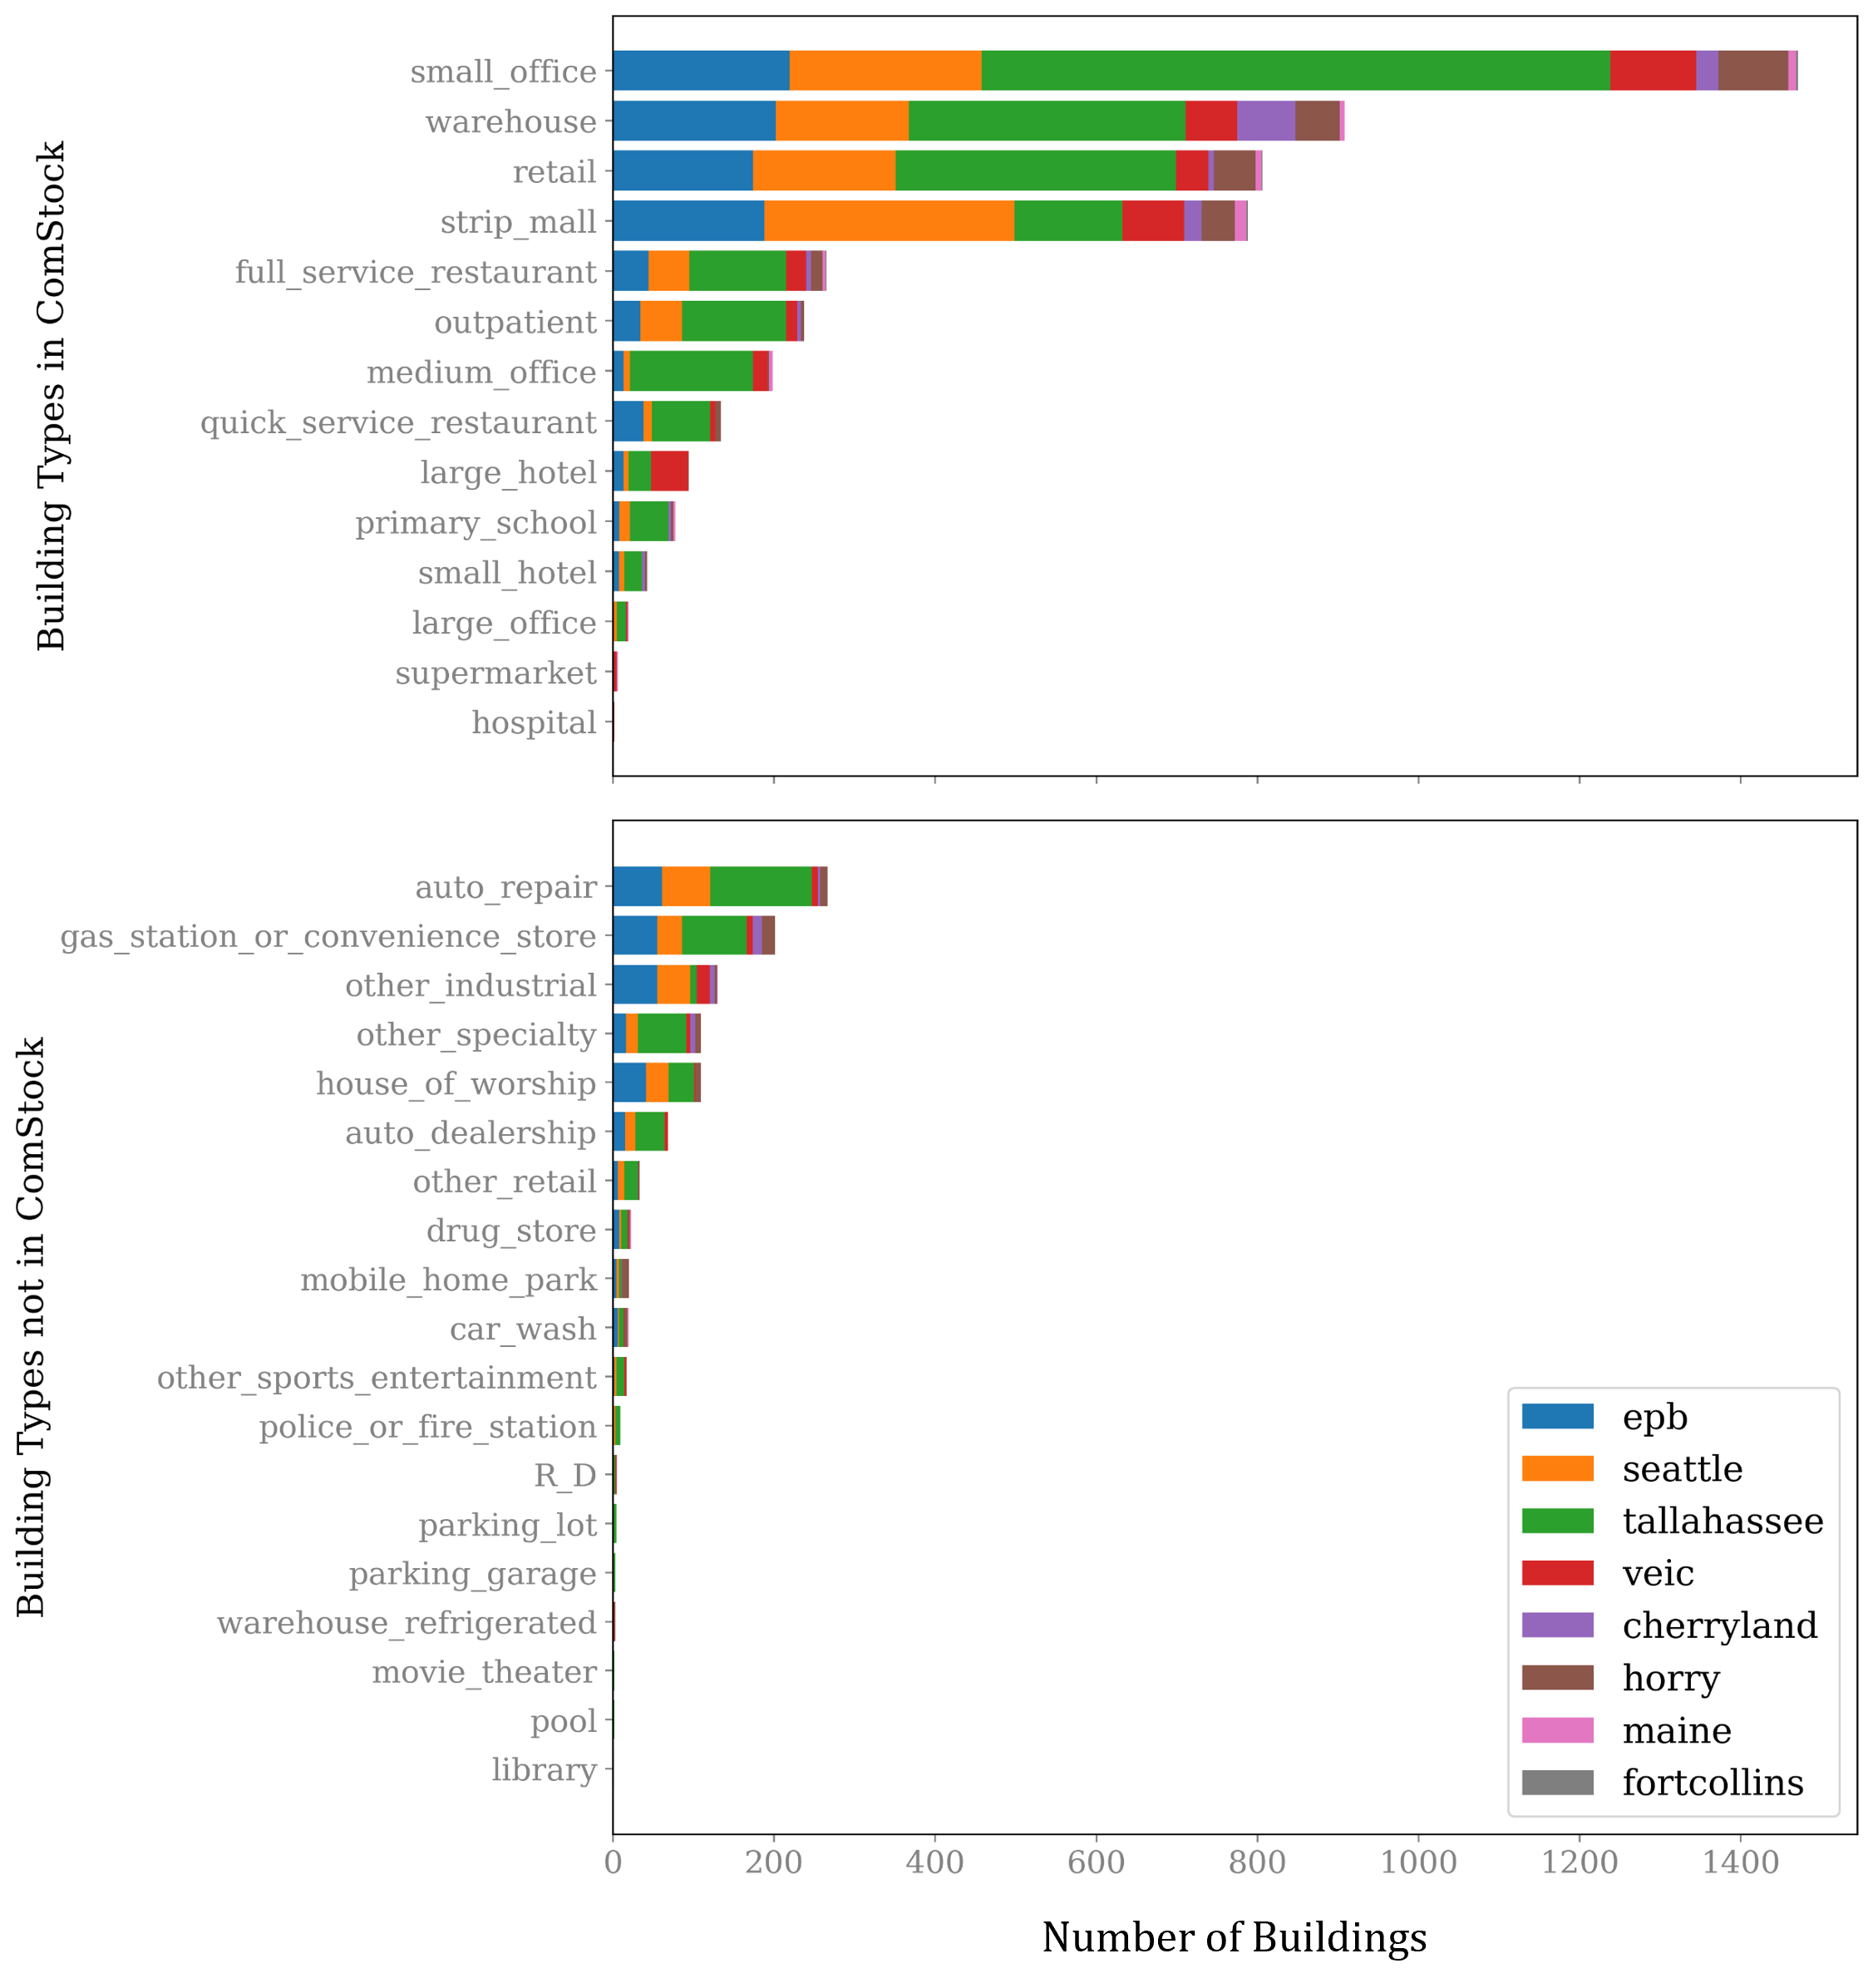
\includegraphics[width=0.8\textwidth]{figures/utility_building_type.png}
    \caption[Number of samples by building type and utility in the commercial AMI data set]{Number of samples by building type and utility in the commercial AMI data set used to derive hours of operation schedules. See EULP Final Technical Report Table 10 for more detail. For example, "epb" is AMI data from Chattanooga, TN.}
    \label{fig:utility_building_type}
\end{figure}

\begin{figure}
    \centering 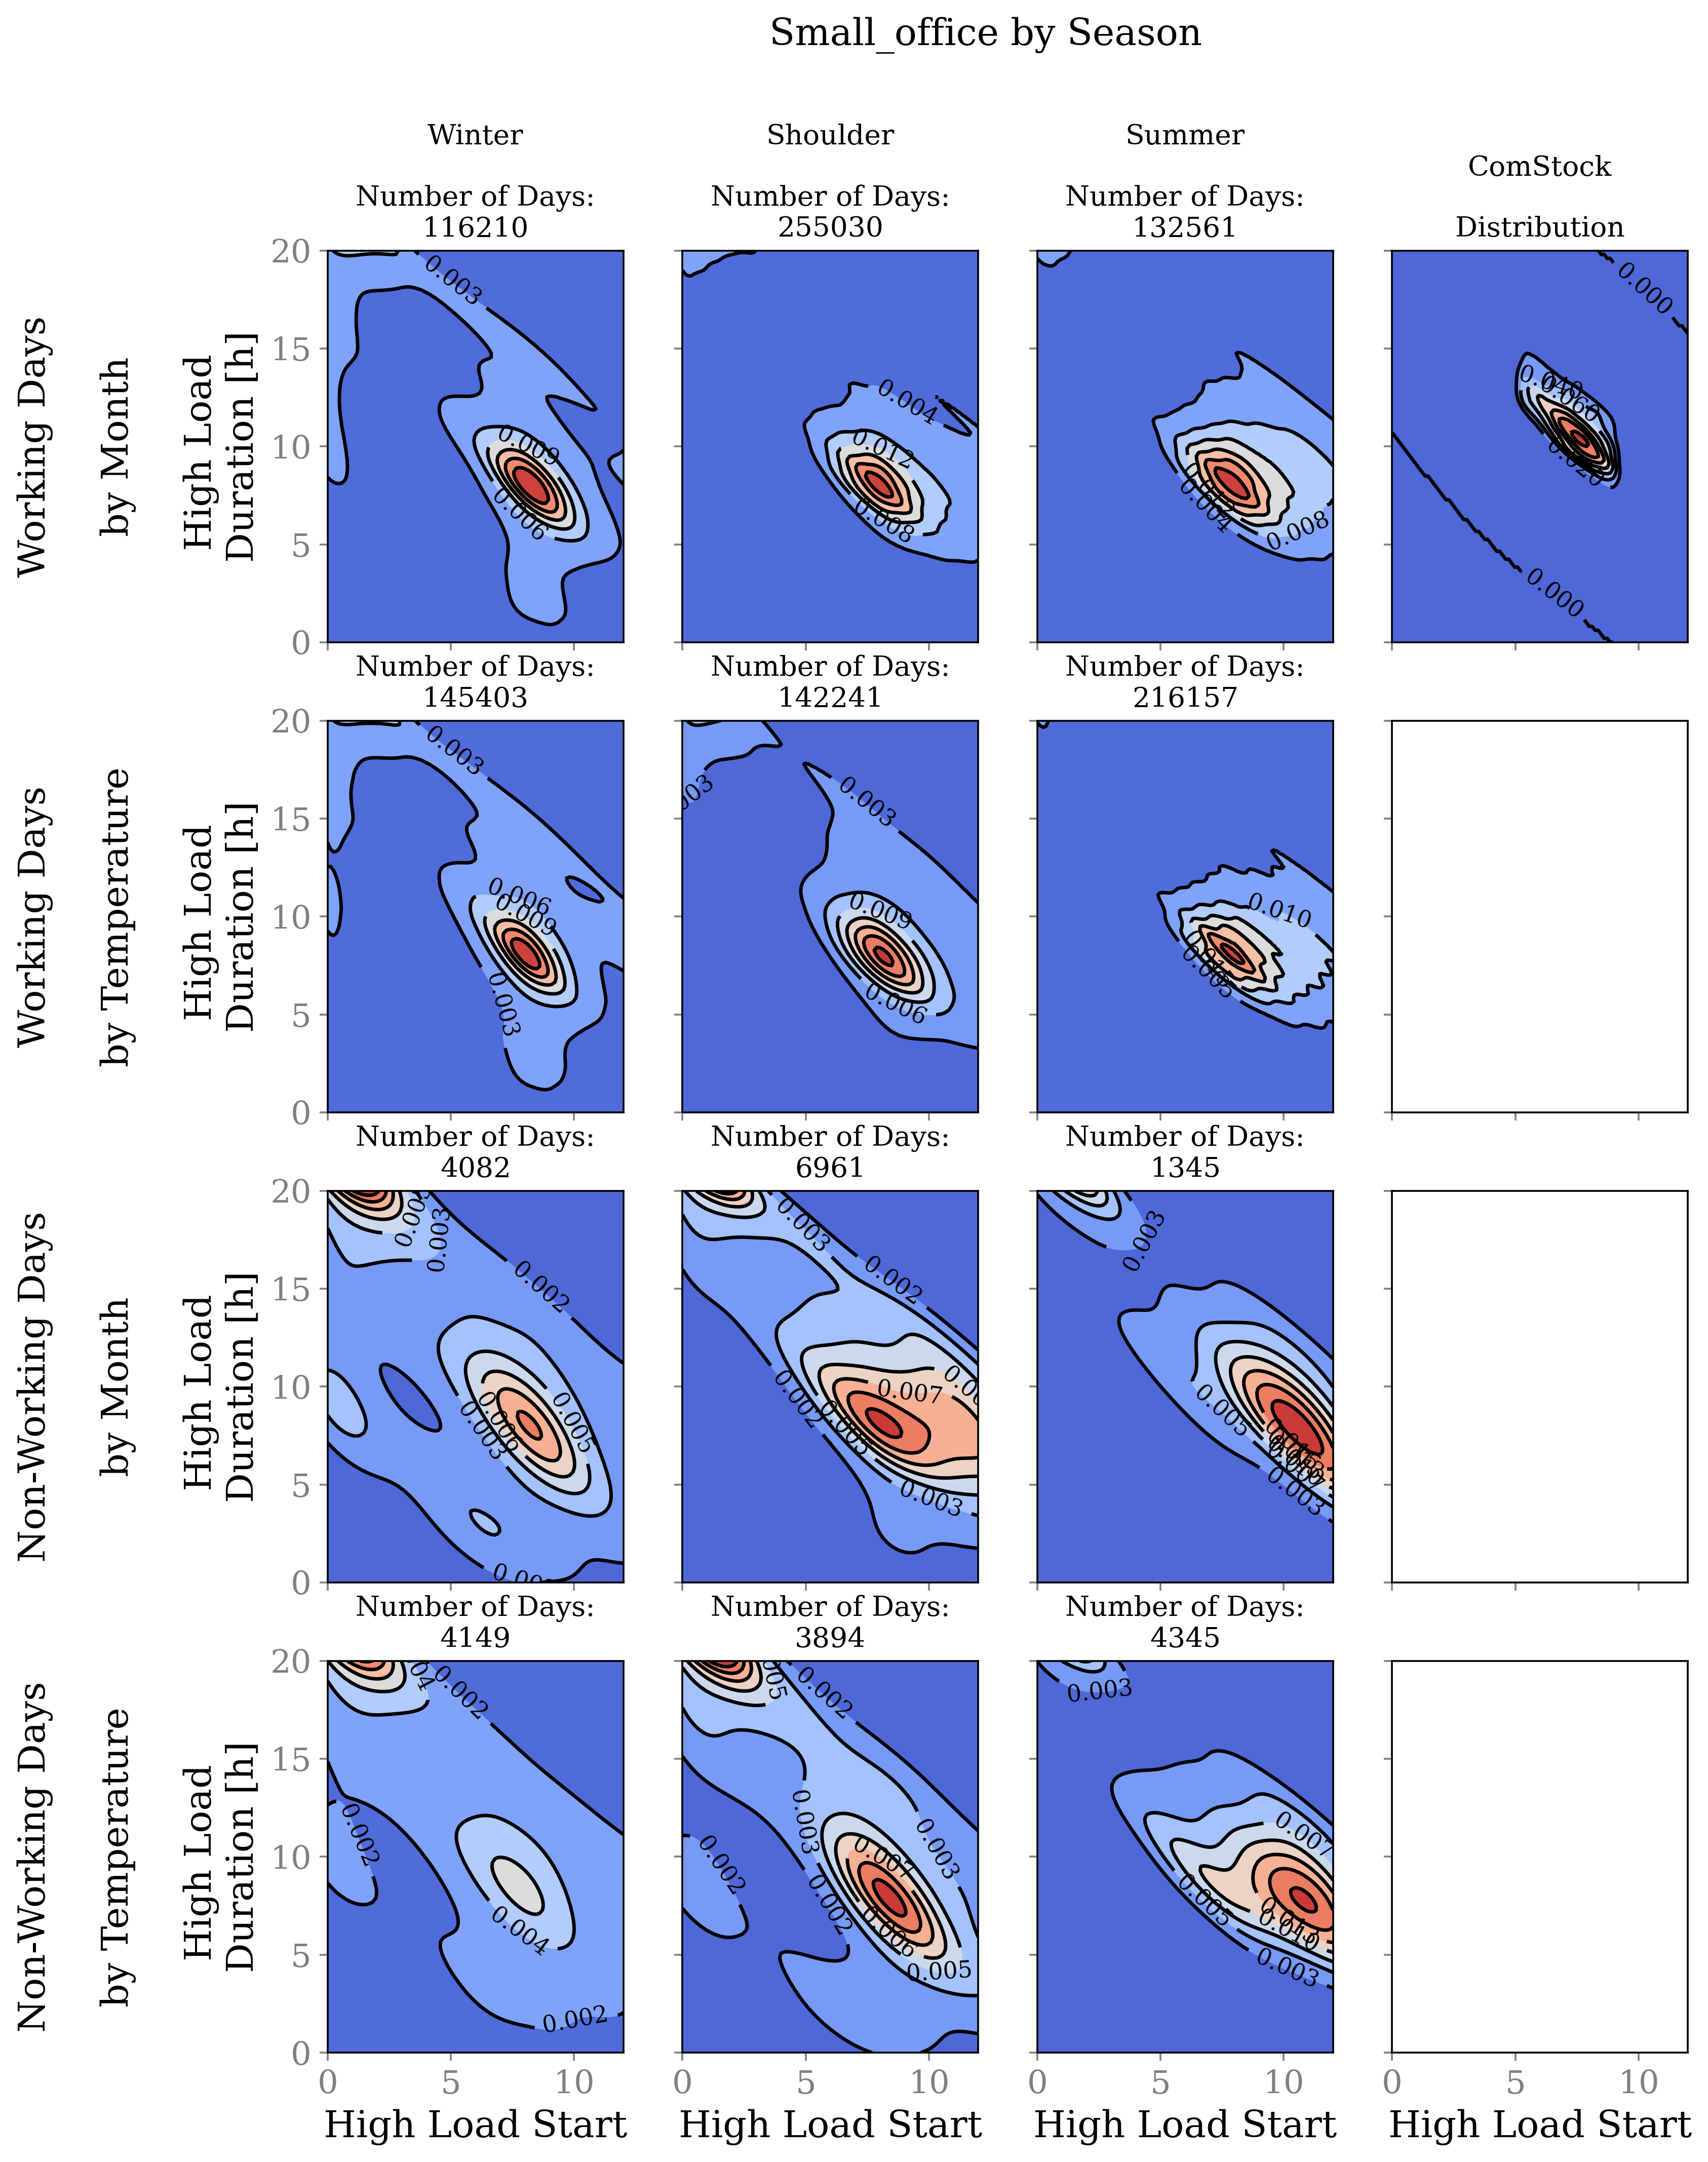
\includegraphics[width=0.8\textwidth]{figures/small_office_season.png}
    \caption[Distribution of small office hours of operations, by day type and season]{Distribution of small office hours of operations extracted from AMI data (from seven utilities), by day type and season, and compared to ComStock before updates. This figure shows how the hours of operation (start time and duration of the high load period) are influenced by season (all utilities are combined in this plot).}
    \label{fig:small_office_season}
\end{figure}

\begin{figure}
    \centering 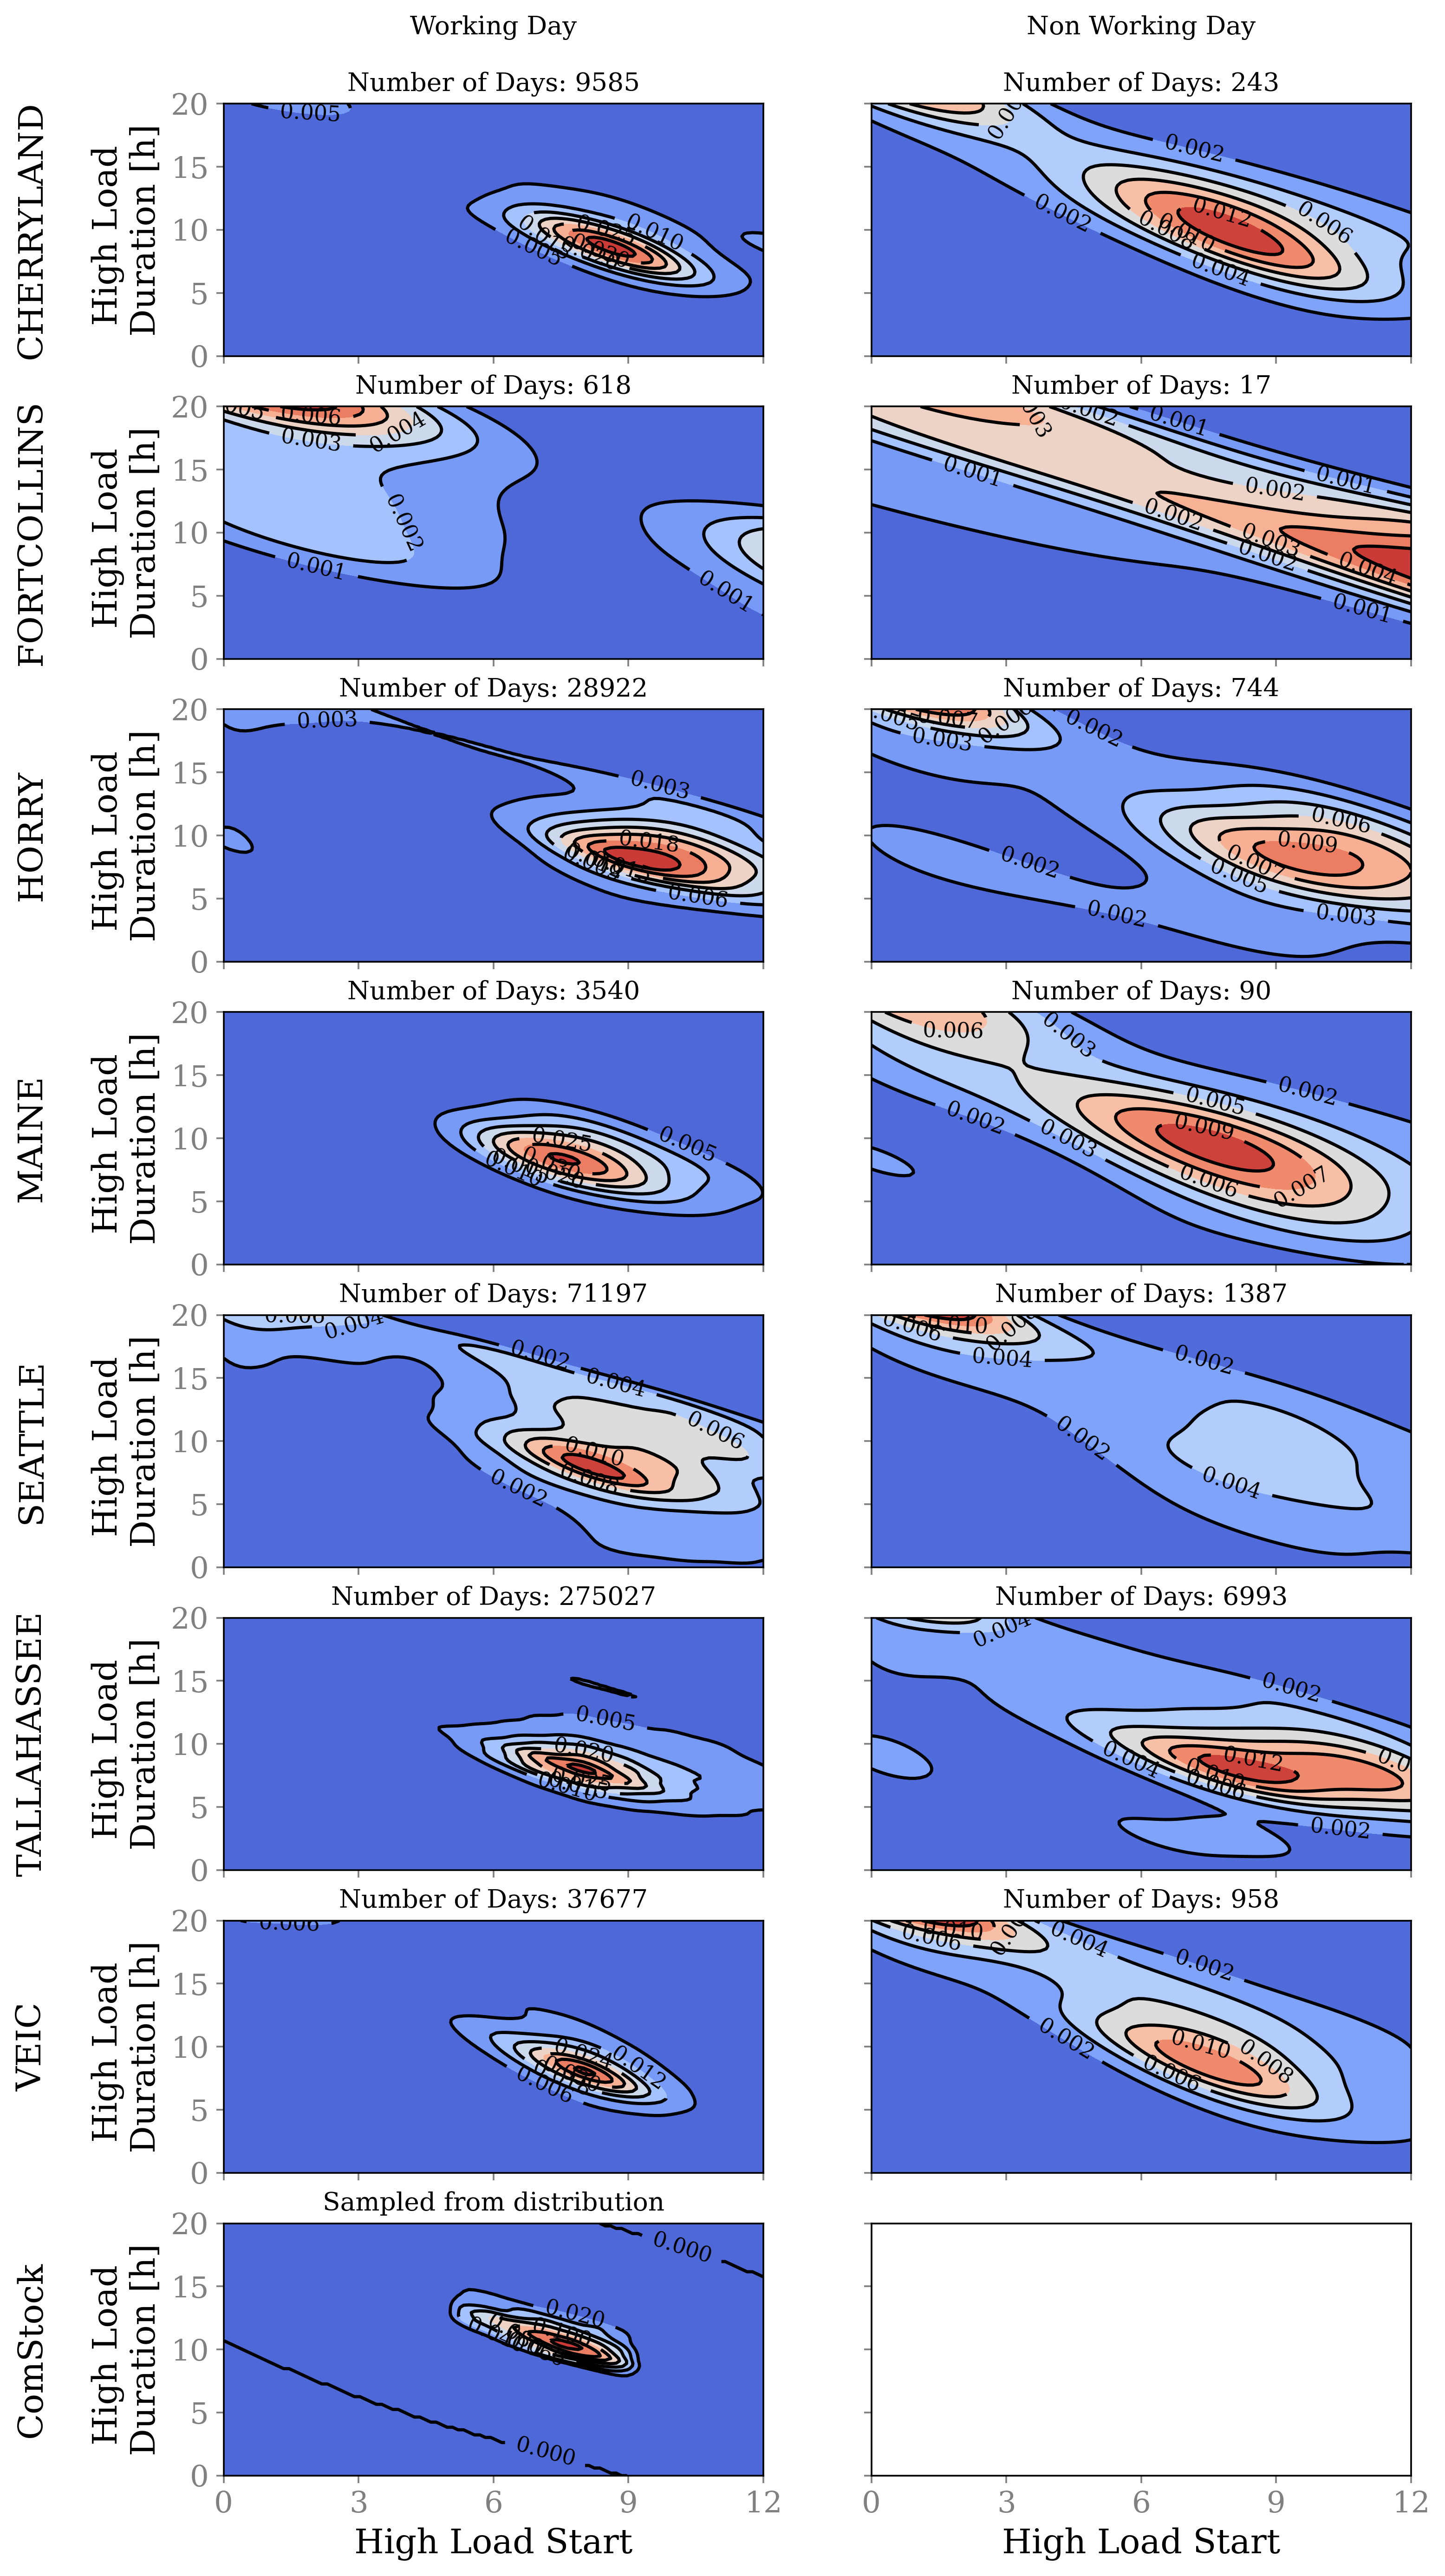
\includegraphics[width=0.7\textwidth]{figures/small_office_utility.png}
    \caption[Distribution of small office hours of operation, by utility and day type]{Distribution of small office hours of operations extracted from AMI data (from seven utilities), by utility and day type, and compared to ComStock before updates. This figure shows how the hours of operation (start time and duration of the high load period) are influenced by utility region (all seasons are combined in this plot).}
    \label{fig:small_office_utility}
\end{figure}

\begin{figure}
    \centering
    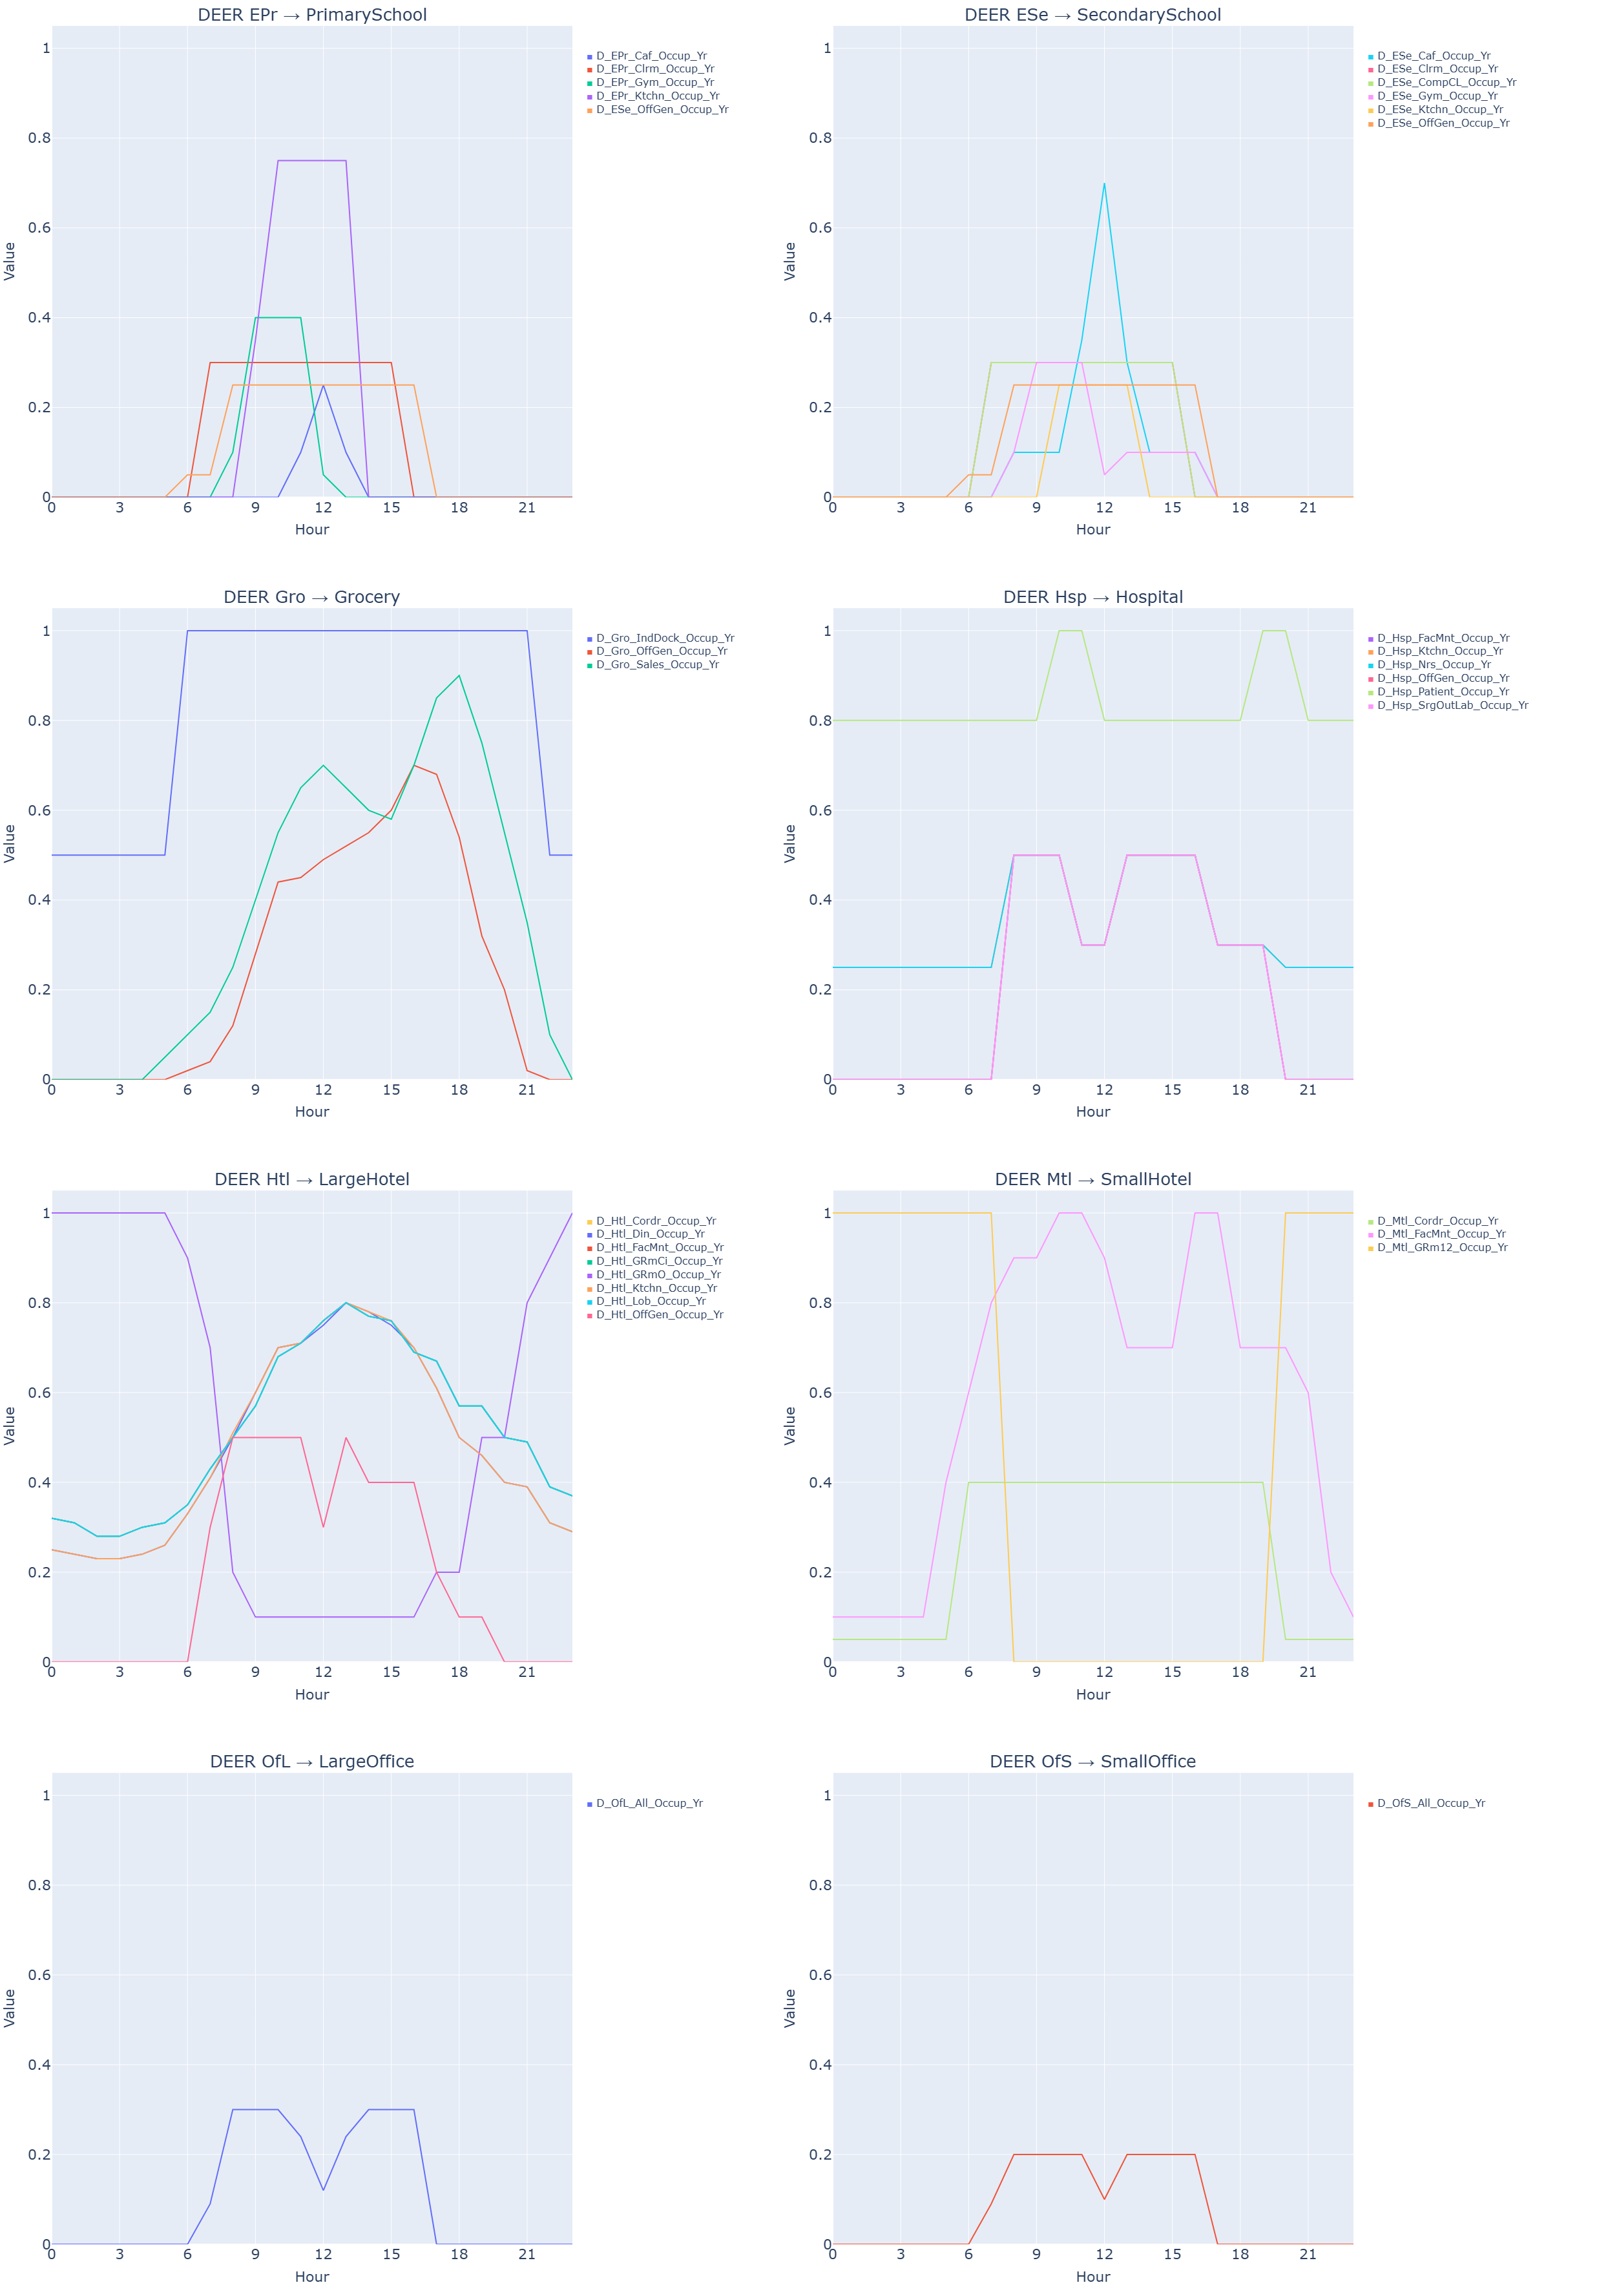
\includegraphics[trim={0 0 0 0}, clip,  % L B R T
    width=\textwidth]{figures/occupancy_schedules_deer_1.png}
    \caption[California base occupancy schedules] {California base occupancy schedules for food service, lodging, healthcare, and education ComStock building types.}
    \label{fig:occupancy_schedules_deer_1}
\end{figure}

\begin{figure}
    \centering
    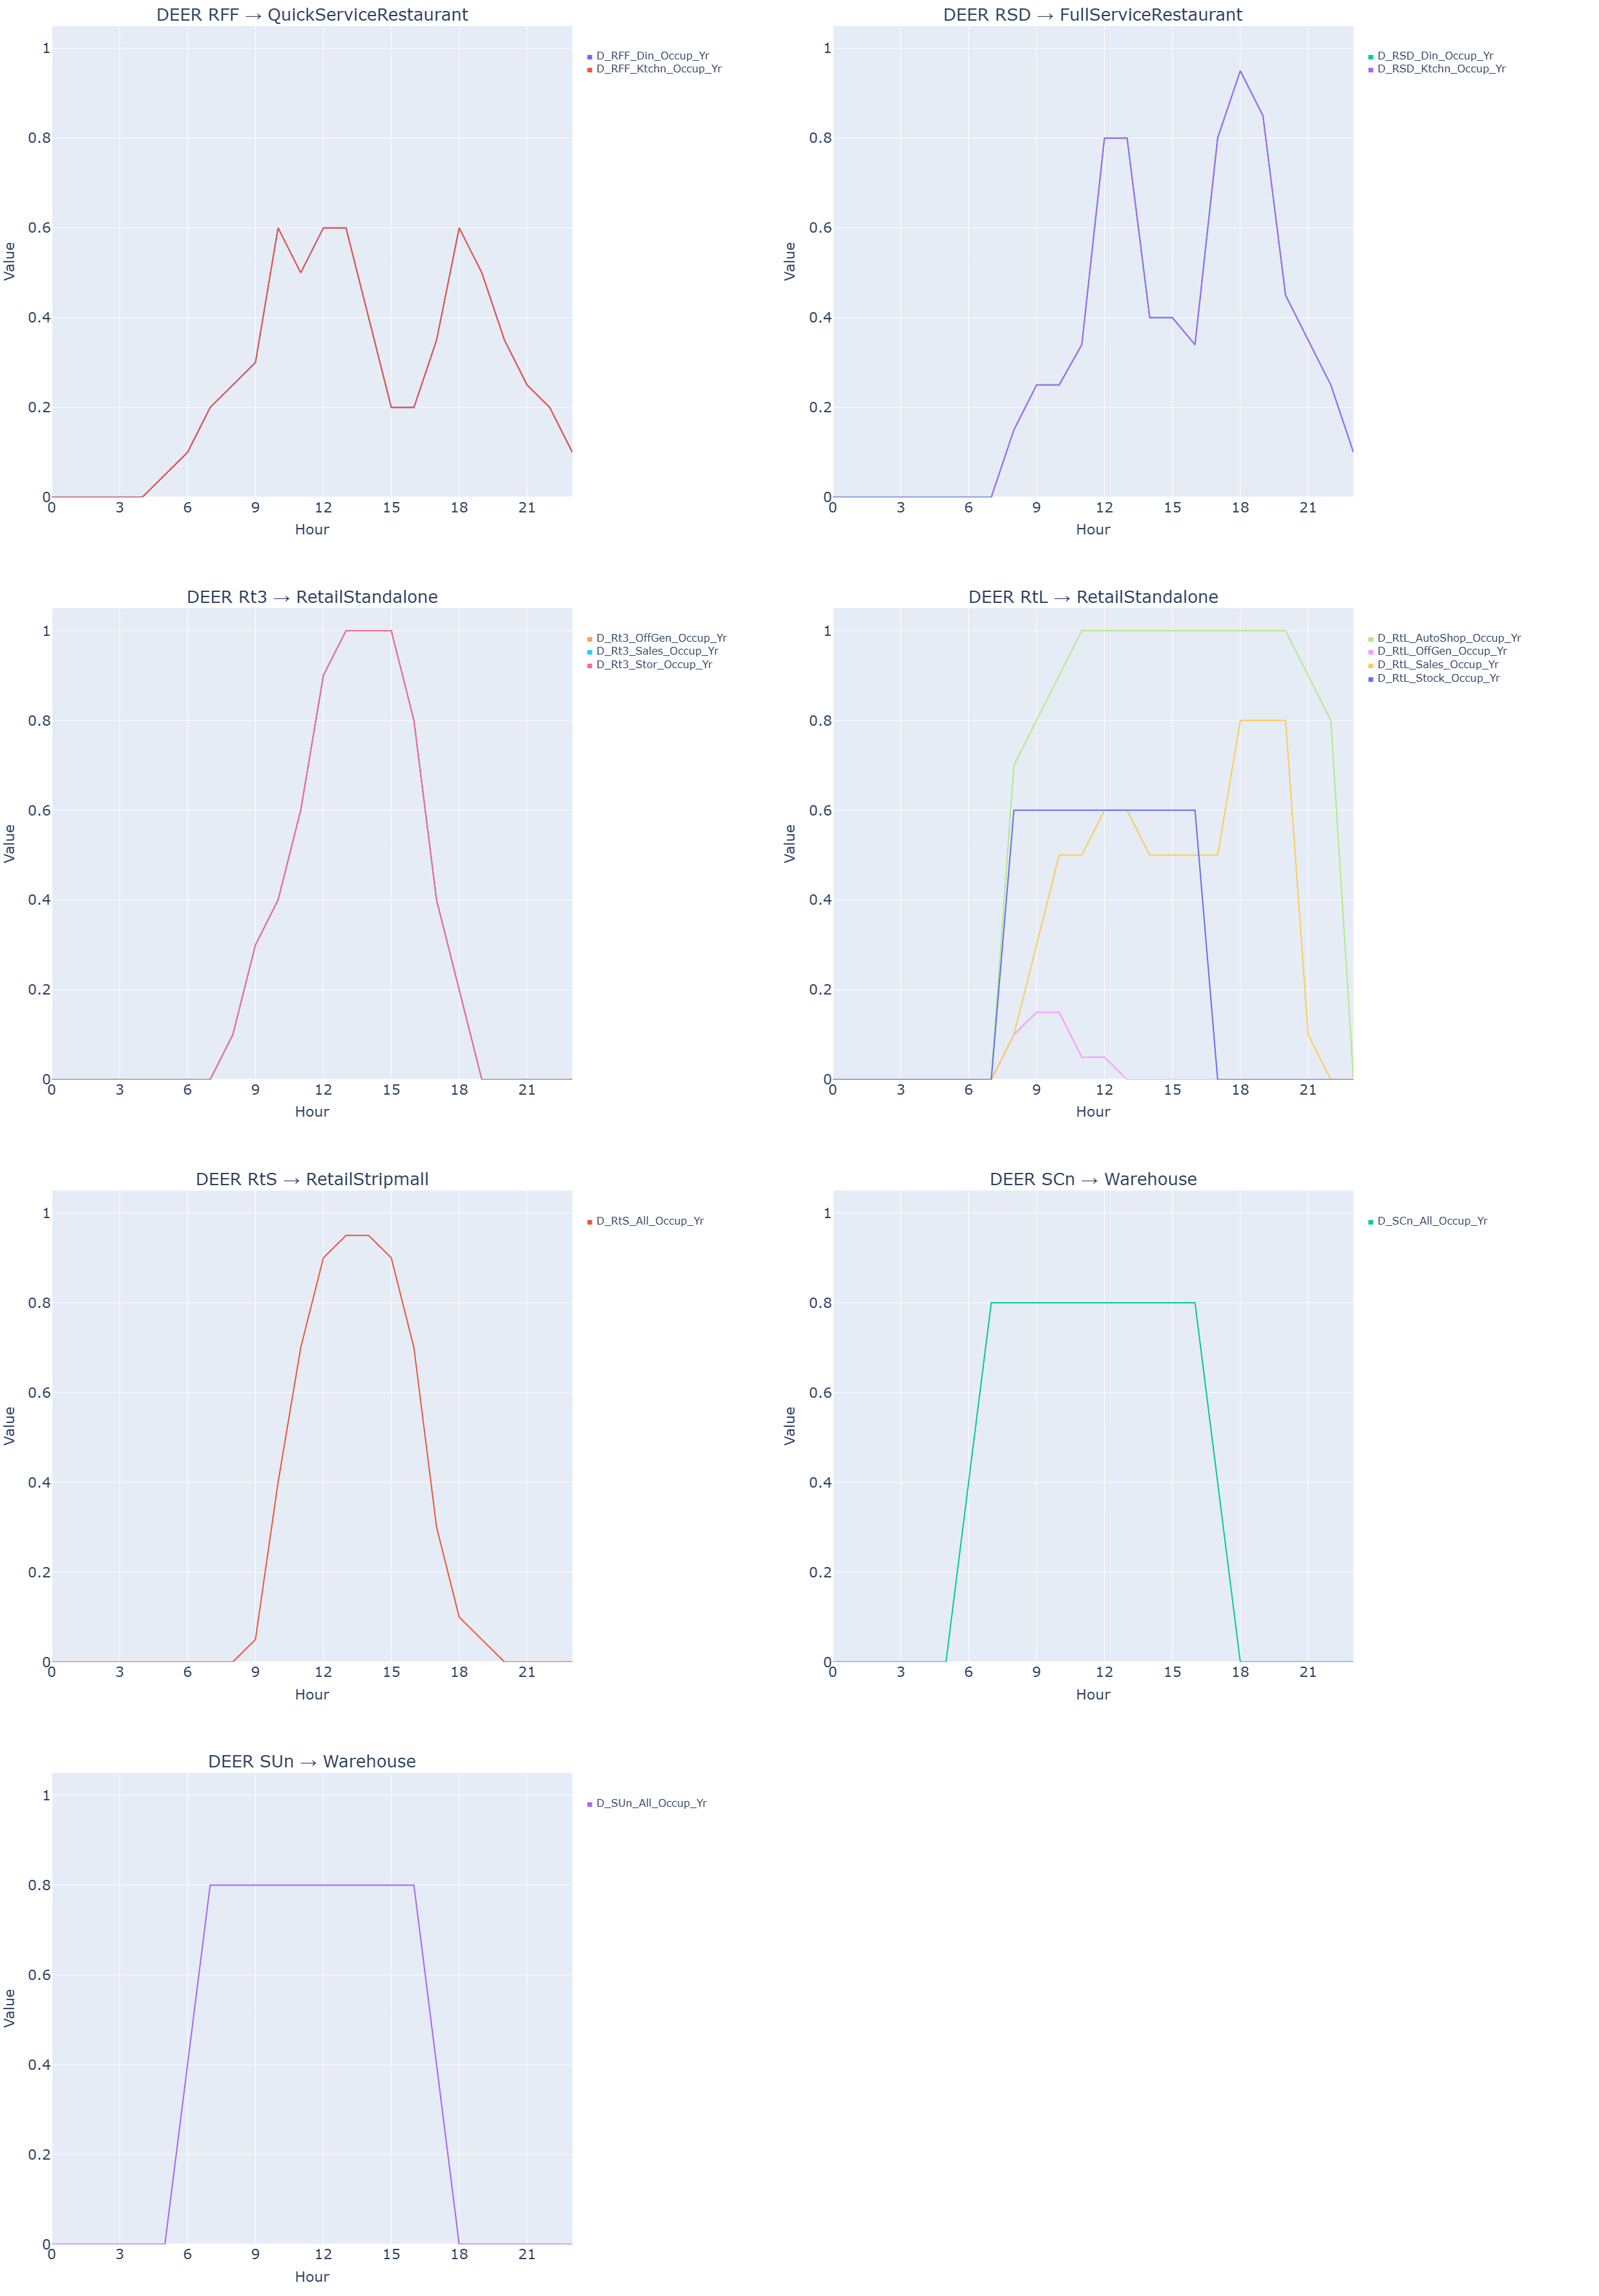
\includegraphics[trim={0 0 0 0}, clip,  % L B R T
    width=\textwidth]{figures/occupancy_schedules_deer_2.png}
    \caption[California base occupancy schedules continued]{California base occupancy schedules for retail, office, and warehouse ComStock building types.}
    \label{fig:occupancy_schedules_deer_2}
\end{figure}

\begin{figure}
  \centering
  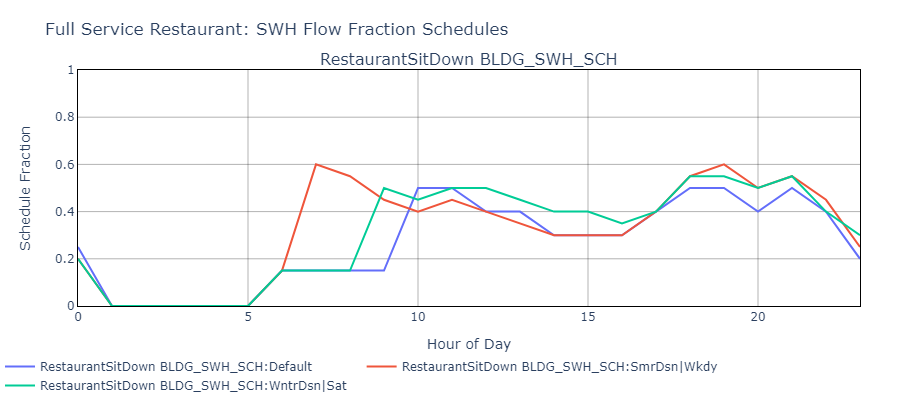
\includegraphics[width=\textwidth]{figures/swh_sched_full service restaurant.png}
  \caption[SWH heating usage schedule for full service restaurants]{SWH heating usage schedule for full service restaurants.}
  \label{fig:swh_sched_fsr}
\end{figure}

\begin{figure}
  \centering
  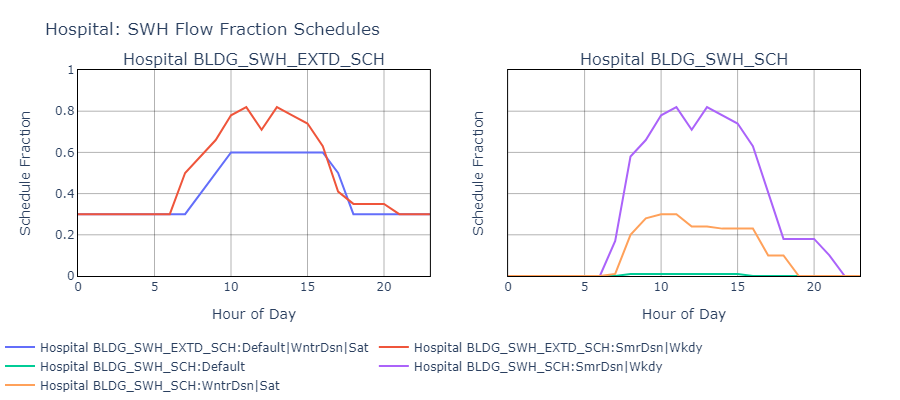
\includegraphics[width=\textwidth]{figures/swh_sched_hospital.png}
  \caption[SWH heating usage schedule for hospitals]{SWH heating usage schedule for hospitals.}
  \label{fig:swh_sched_hos}
\end{figure}

\begin{figure}
  \centering
  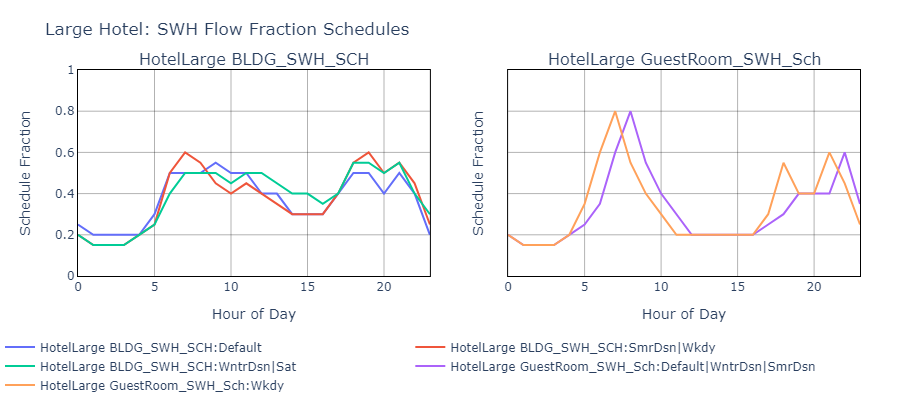
\includegraphics[width=\textwidth]{figures/swh_sched_large hotel.png}
  \caption[SWH heating usage schedule for large hotel]{SWH heating usage schedule for large hotel.}
  \label{fig:swh_sched_large_hotel}
\end{figure}

\begin{figure}
  \centering
  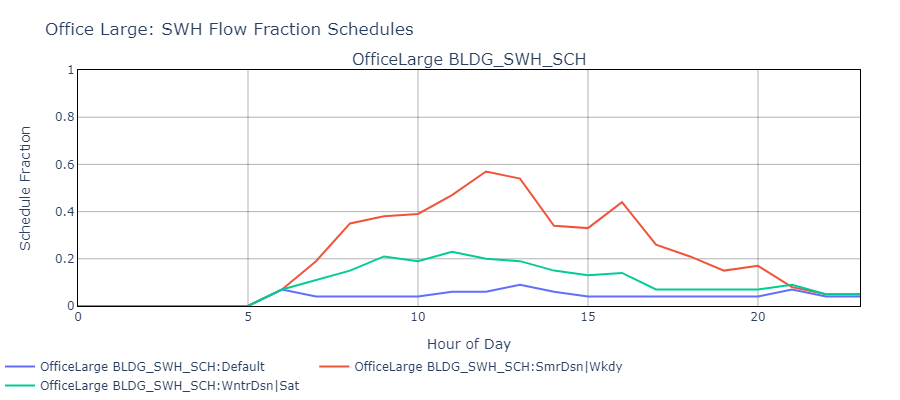
\includegraphics[width=\textwidth]{figures/swh_sched_office large.png}
  \caption[SWH heating usage schedule for large office]{SWH heating usage schedule for large office.}
  \label{fig:swh_sched_large_office}
\end{figure}

\begin{figure}
  \centering
  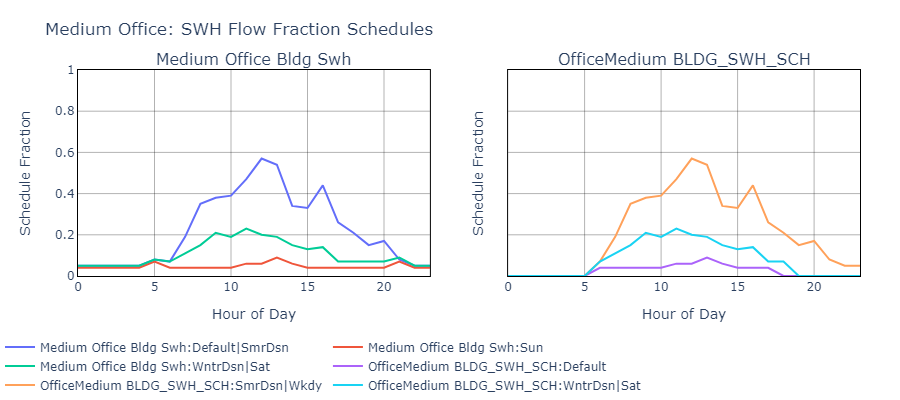
\includegraphics[width=\textwidth]{figures/swh_sched_medium office.png}
  \caption[SWH heating usage schedule for medium office]{SWH heating usage schedule for medium office.}
  \label{fig:swh_sched_medium_office}
\end{figure}

\begin{figure}
  \centering
  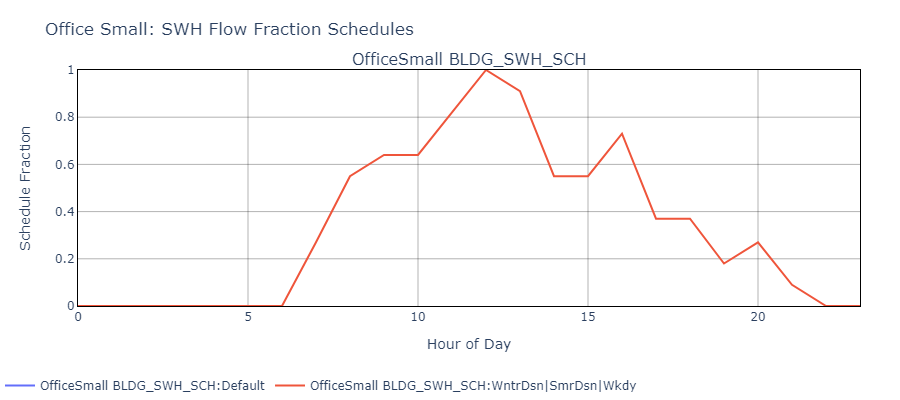
\includegraphics[width=\textwidth]{figures/swh_sched_office small.png}
  \caption[SWH heating usage schedule for small offices]{SWH heating usage schedule for small offices.}
  \label{fig:swh_sched_small_office}
\end{figure}

\begin{figure}
  \centering
  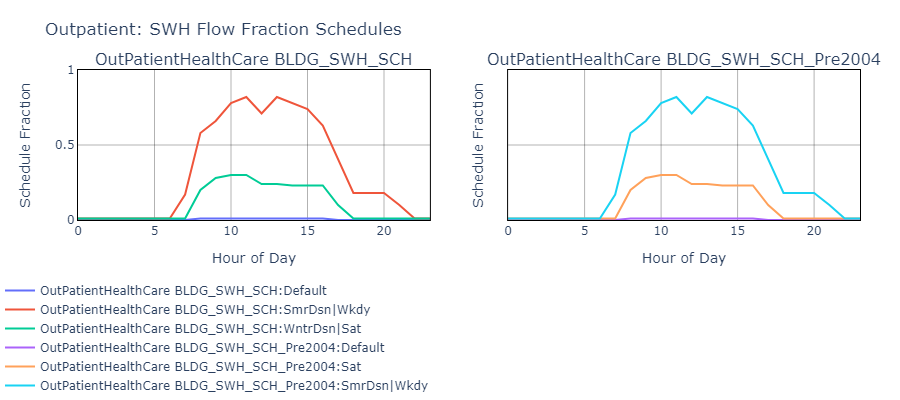
\includegraphics[width=\textwidth]{figures/swh_sched_outpatient.png}
  \caption[SWH heating usage schedule for outpatient]{SWH heating usage schedule for outpatient.}
  \label{fig:swh_sched_outpatient}
\end{figure}

\begin{figure}
  \centering
  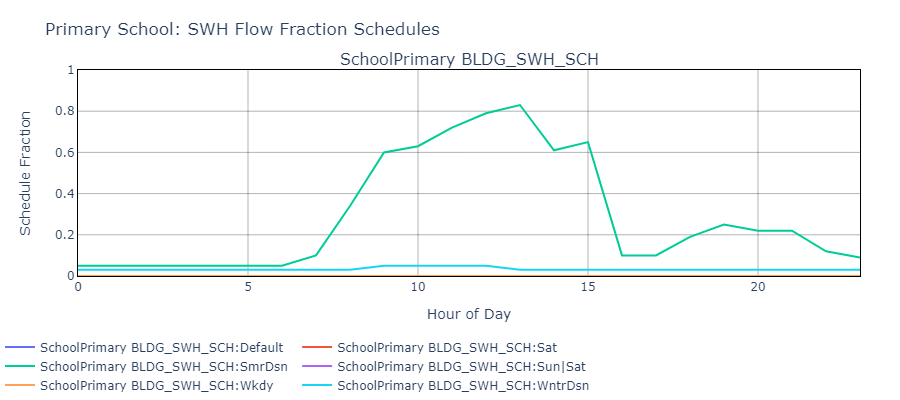
\includegraphics[width=\textwidth]{figures/swh_sched_primary school.png}
  \caption[SWH heating usage schedule for primary school]{SWH heating usage schedule for primary school.}
  \label{fig:swh_sched_primary_school}
\end{figure}

\begin{figure}
  \centering
  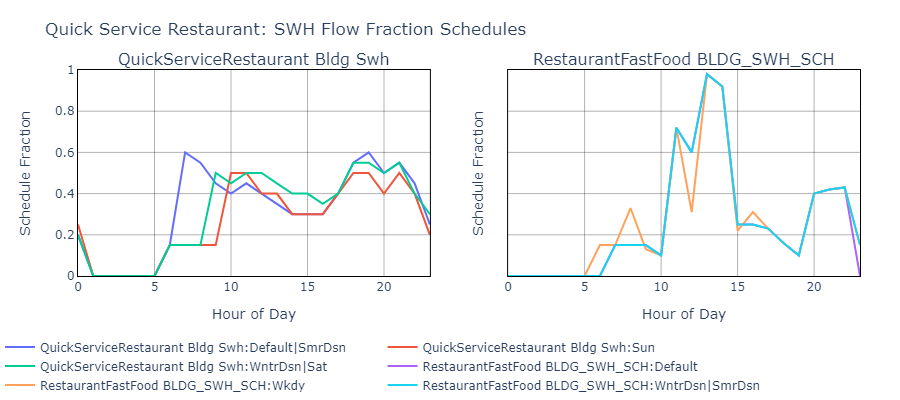
\includegraphics[width=\textwidth]{figures/swh_sched_quick service restaurant.png}
  \caption[SWH heating usage schedule for quick service restaurant]{SWH heating usage schedule for quick service restaurant.}
  \label{fig:swh_sched_quick_service_restaurant}
\end{figure}

\begin{figure}
  \centering
  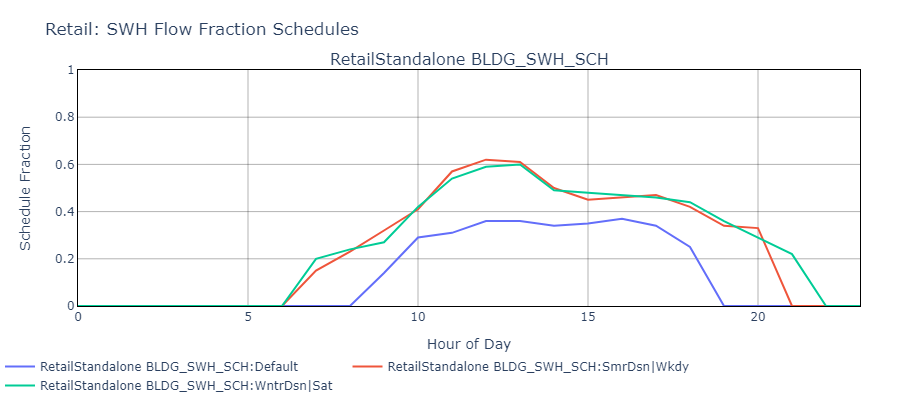
\includegraphics[width=\textwidth]{figures/swh_sched_retail.png}
  \caption[SWH heating usage schedule for retail]{SWH heating usage schedule for retail.}
  \label{fig:swh_sched_retail}
\end{figure}

\begin{figure}
  \centering
  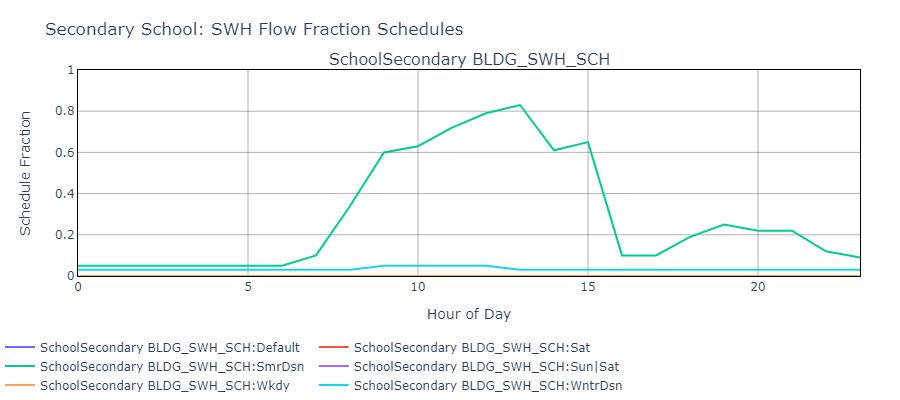
\includegraphics[width=\textwidth]{figures/swh_sched_secondary school.png}
  \caption[SWH heating usage schedule for secondary school]{SWH heating usage schedule for secondary school.}
  \label{fig:swh_sched_secondary_school}
\end{figure}

\begin{figure}
  \centering
  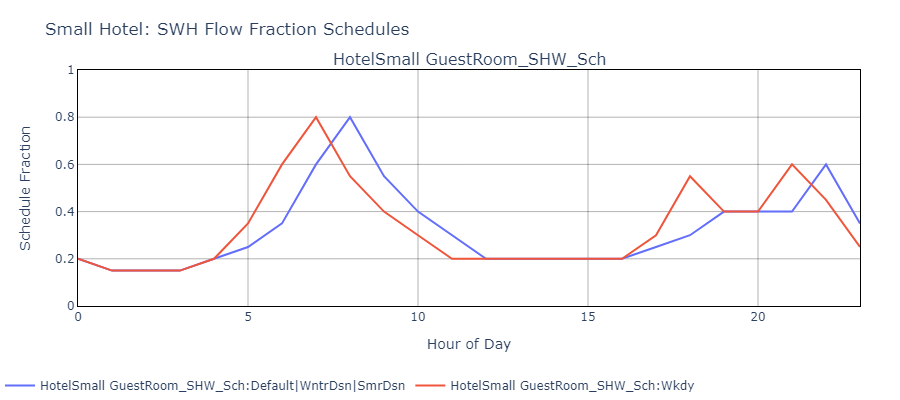
\includegraphics[width=\textwidth]{figures/swh_sched_small hotel.png}
  \caption[SWH heating usage schedule for small hotel]{SWH heating usage schedule for small hotel.}
  \label{fig:swh_sched_small_hotel}
\end{figure}

\begin{figure}
  \centering
  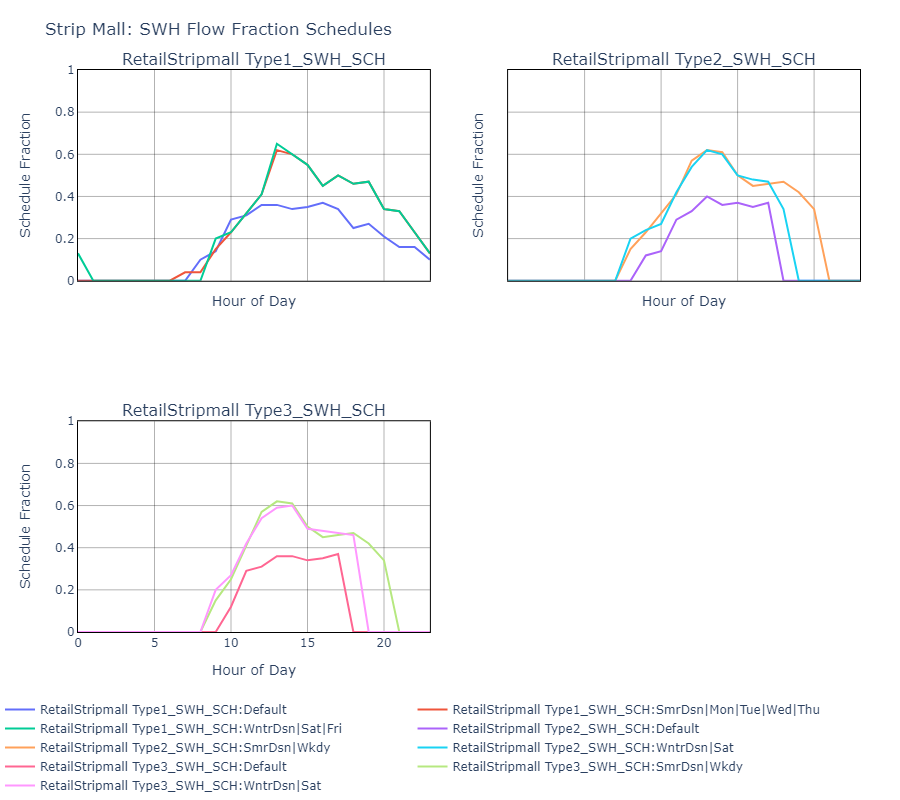
\includegraphics[width=\textwidth]{figures/swh_sched_strip mall.png}
  \caption[SWH heating usage schedule for strip mall]{SWH heating usage schedule for strip mall.}
  \label{fig:swh_sched_strip_mall}
\end{figure}

% \begin{figure}
%   \centering
%   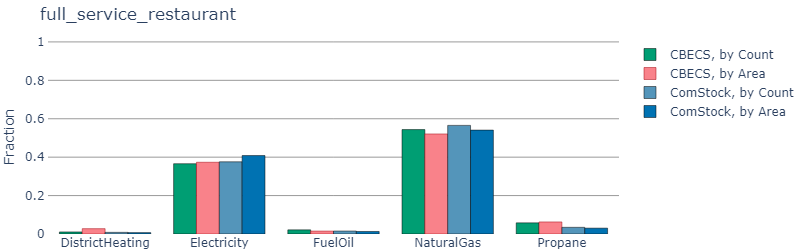
\includegraphics[scale=0.5]{figures/cbecs_comstock_fuel_comparison_full_service_restaurant.png}
%   \caption[Comparison of fuel type prevalence between ComStock and CBECS for full service restaurants]{Area-weighted vs. building-count-weighted comparison of fuel type prevalence between ComStock and CBECS for full service restaurants. From left to right, the fuel types on the x-axis are: district heating, electricity, fuel oil, natural gas, and propane.}
% \label{fig:cbecs_comstock_fuel_comparison_full_service_restaurant}
% \end{figure}

% \begin{figure}
%   \centering
%   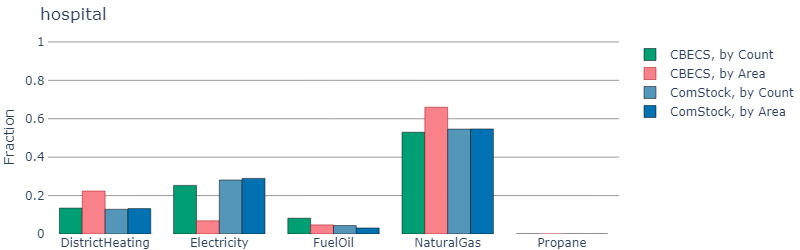
\includegraphics[scale=0.5]{figures/cbecs_comstock_fuel_comparison_hospital.png}
%   \caption[Comparison of fuel type prevalence between ComStock and CBECS for hospitals]{Area-weighted vs. building-count-weighted comparison of fuel type prevalence between ComStock and CBECS for hospitals. From left to right, the fuel types on the x-axis are: district heating, electricity, fuel oil, natural gas, and propane.}
%   \label{fig:cbecs_comstock_fuel_comparison_hospital}
% \end{figure}

% \begin{figure}
%   \centering
%   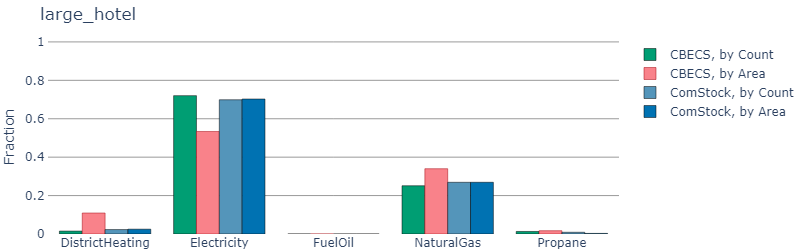
\includegraphics[scale=0.5]{figures/cbecs_comstock_fuel_comparison_large_hotel.png}
%   \caption[Comparison of fuel type prevalence between ComStock and CBECS for large hotels]{Area-weighted vs. building-count-weighted comparison of fuel type prevalence between ComStock and CBECS for large hotels. From left to right, the fuel types on the x-axis are: district heating, electricity, fuel oil, natural gas, and propane.}
%   \label{fig:cbecs_comstock_fuel_comparison_large_hotel}
% \end{figure}

% \begin{figure}
%   \centering
%   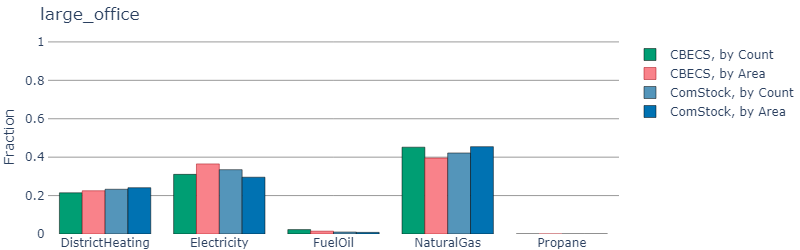
\includegraphics[scale=0.5]{figures/cbecs_comstock_fuel_comparison_large_office.png}
%   \caption[Comparison of fuel type prevalence between ComStock and CBECS for large offices]{Area-weighted vs. building-count-weighted comparison of fuel type prevalence between ComStock and CBECS for large offices. From left to right, the fuel types on the x-axis are: district heating, electricity, fuel oil, natural gas, and propane.}
%   \label{fig:cbecs_comstock_fuel_comparison_large_office}
% \end{figure}

% \begin{figure}
%   \centering
%   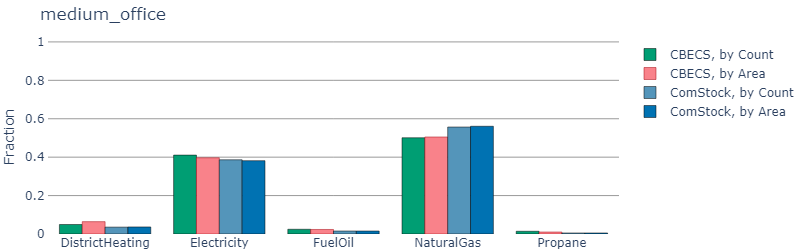
\includegraphics[scale=0.5]{figures/cbecs_comstock_fuel_comparison_medium_office.png}
%   \caption[Comparison of fuel type prevalence between ComStock and CBECS for medium offices]{Area-weighted vs. building-count-weighted comparison of fuel type prevalence between ComStock and CBECS for medium offices. From left to right, the fuel types on the x-axis are: district heating, electricity, fuel oil, natural gas, and propane.}
%   \label{fig:cbecs_comstock_fuel_comparison_medium_office}
% \end{figure}

% \begin{figure}
%   \centering
%   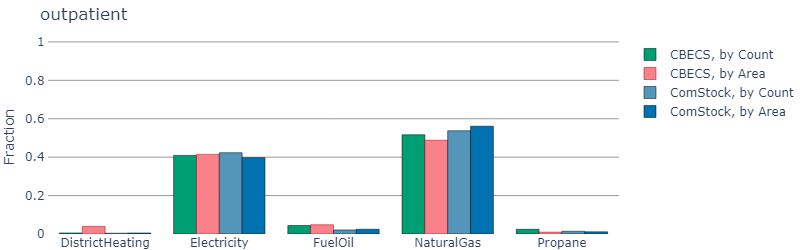
\includegraphics[scale=0.5]{figures/cbecs_comstock_fuel_comparison_outpatient.png}
%   \caption[Comparison of fuel type prevalence between ComStock and CBECS for outpatient]{Area-weighted vs. building-count-weighted comparison of fuel type prevalence between ComStock and CBECS for outpatient. From left to right, the fuel types on the x-axis are: district heating, electricity, fuel oil, natural gas, and propane.}
%   \label{fig:cbecs_comstock_fuel_comparison_outpatient}
% \end{figure}

% \begin{figure}
%   \centering
%   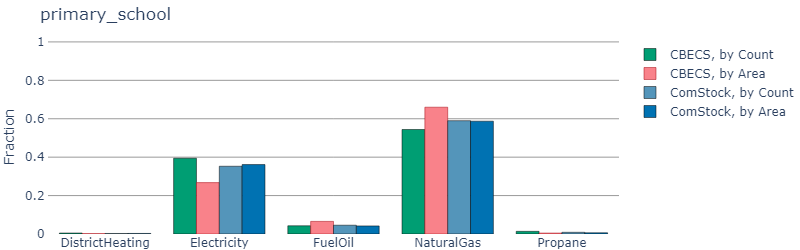
\includegraphics[scale=0.5]{figures/cbecs_comstock_fuel_comparison_primary_school.png}
%   \caption[Comparison of fuel type prevalence between ComStock and CBECS for primary schools]{Area-weighted vs. building-count-weighted comparison of fuel type prevalence between ComStock and CBECS for primary schools. From left to right, the fuel types on the x-axis are: district heating, electricity, fuel oil, natural gas, and propane.}
%   \label{fig:cbecs_comstock_fuel_comparison_primary_school}
% \end{figure}

% \begin{figure}
%   \centering
%   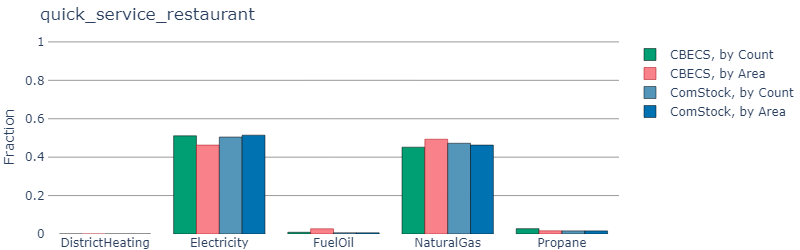
\includegraphics[scale=0.5]{figures/cbecs_comstock_fuel_comparison_quick_service_restaurant.png}
%   \caption[Comparison of fuel type prevalence between ComStock and CBECS for quick service restaurants]{Area-weighted vs. building-count-weighted comparison of fuel type prevalence between ComStock and CBECS for quick service restaurants. From left to right, the fuel types on the x-axis are: district heating, electricity, fuel oil, natural gas, and propane.}
%   \label{fig:cbecs_comstock_fuel_comparison_quick_service_restaurant}
% \end{figure}

% \begin{figure}
%   \centering
%   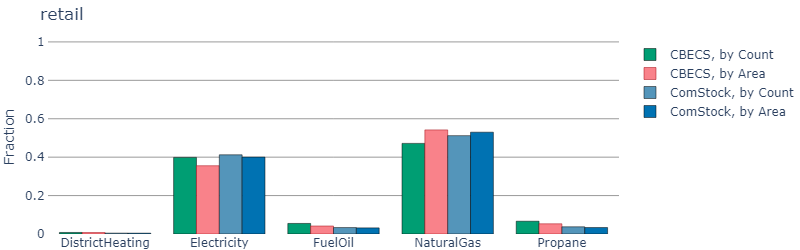
\includegraphics[scale=0.5]{figures/cbecs_comstock_fuel_comparison_retail.png}
%   \caption[Comparison of fuel type prevalence between ComStock and CBECS for retail]{Area-weighted vs. building-count-weighted comparison of fuel type prevalence between ComStock and CBECS for retail. From left to right, the fuel types on the x-axis are: district heating, electricity, fuel oil, natural gas, and propane.}
%   \label{fig:cbecs_comstock_fuel_comparison_retail}
% \end{figure}

% \begin{figure}
%   \centering
%   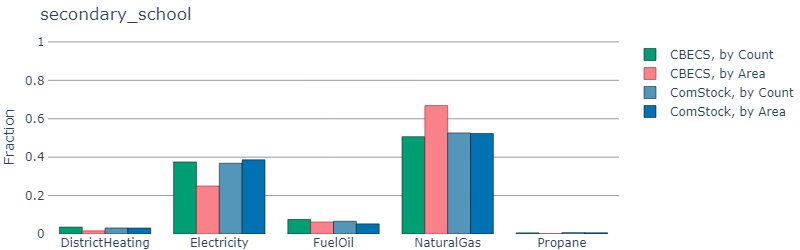
\includegraphics[scale=0.5]{figures/cbecs_comstock_fuel_comparison_secondary_school.png}
%   \caption[Comparison of fuel type prevalence between ComStock and CBECS for secondary schools]{Area-weighted vs. building-count-weighted comparison of fuel type prevalence between ComStock and CBECS for secondary schools. From left to right, the fuel types on the x-axis are: district heating, electricity, fuel oil, natural gas, and propane.}
%   \label{fig:cbecs_comstock_fuel_comparison_secondary_school}
% \end{figure}

% \begin{figure}
%   \centering
%   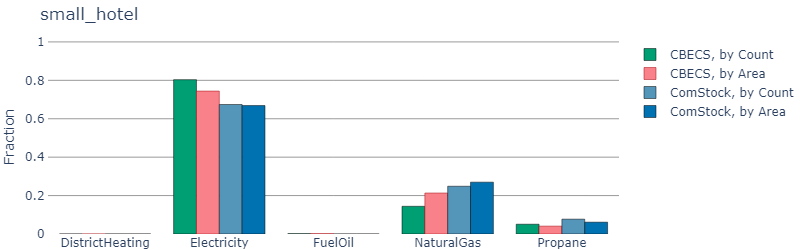
\includegraphics[scale=0.5]{figures/cbecs_comstock_fuel_comparison_small_hotel.png}
%   \caption[Comparison of fuel type prevalence between ComStock and CBECS for small hotel]{Area-weighted vs. building-count-weighted comparison of fuel type prevalence between ComStock and CBECS for small hotel. From left to right, the fuel types on the x-axis are: district heating, electricity, fuel oil, natural gas, and propane.}
%   \label{fig:cbecs_comstock_fuel_comparison_small_hotel}
% \end{figure}

% \begin{figure}
%   \centering
%   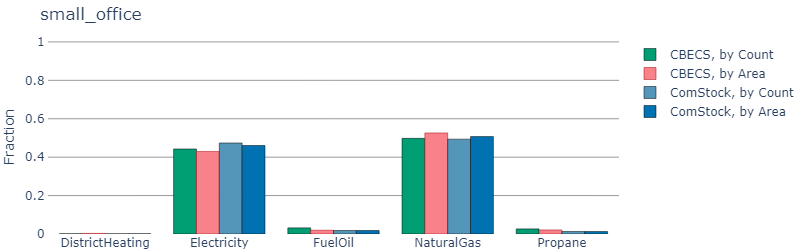
\includegraphics[scale=0.5]{figures/cbecs_comstock_fuel_comparison_small_office.png}
%   \caption[Comparison of fuel type prevalence between ComStock and CBECS for small office]{Area-weighted vs. building-count-weighted comparison of fuel type prevalence between ComStock and CBECS for small office. From left to right, the fuel types on the x-axis are: district heating, electricity, fuel oil, natural gas, and propane.}
%   \label{fig:cbecs_comstock_fuel_comparison_small_office}
% \end{figure}

% \begin{figure}
%   \centering
%   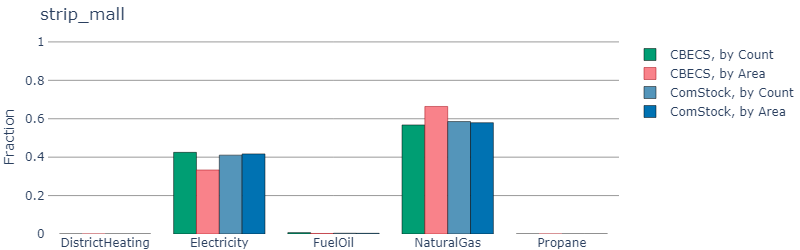
\includegraphics[scale=0.5]{figures/cbecs_comstock_fuel_comparison_strip_mall.png}
%   \caption[Comparison of fuel type prevalence between ComStock and CBECS for strip malls]{Area-weighted vs. building-count-weighted comparison of fuel type prevalence between ComStock and CBECS for strip malls. From left to right, the fuel types on the x-axis are: district heating, electricity, fuel oil, natural gas, and propane.}
%   \label{fig:cbecs_comstock_fuel_comparison_strip_mall}
% \end{figure}

% \begin{figure}
%   \centering
%   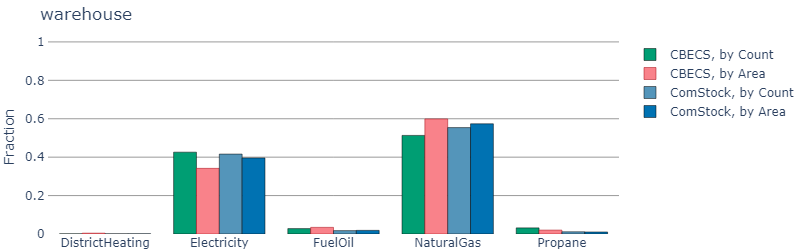
\includegraphics[scale=0.5]{figures/cbecs_comstock_fuel_comparison_warehouse.png}
%   \caption[Comparison of fuel type prevalence between ComStock and CBECS for warehouses]{Area-weighted vs. building-count-weighted comparison of fuel type prevalence between ComStock and CBECS for warehouses. From left to right, the fuel types on the x-axis are: district heating, electricity, fuel oil, natural gas, and propane.}
%   \label{fig:cbecs_comstock_fuel_comparison_warehouse}
% \end{figure}

\begin{figure}
    \centering 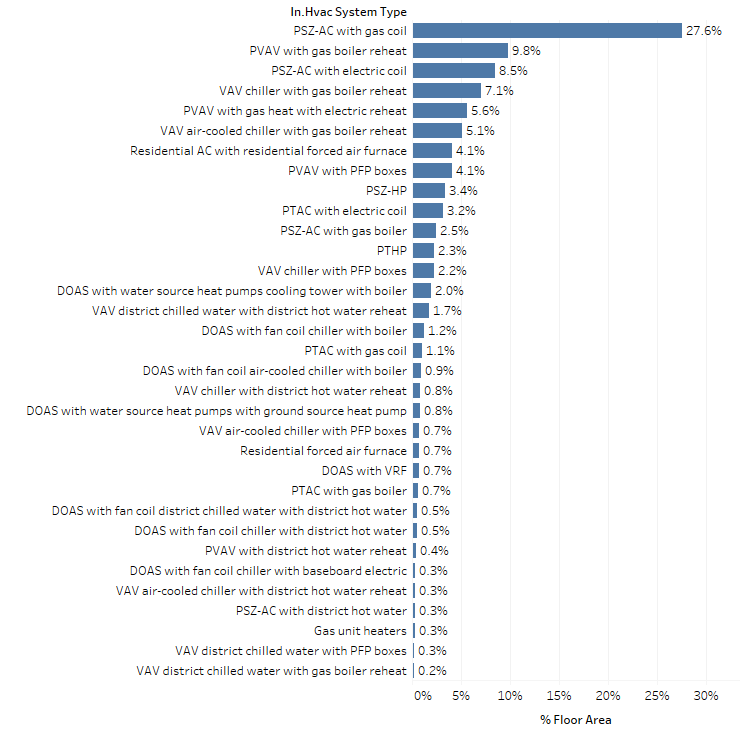
\includegraphics[width=1.0\textwidth]{figures/hvac_system_type_prevalance.png}
    \caption[HVAC system type prevalence in all building types]{Prevalence of ComStock HVAC system types by total stock floor area; all building types.}
    \label{fig:hvac_sys_type_prevalence}
\end{figure}

\begin{figure}
    \centering 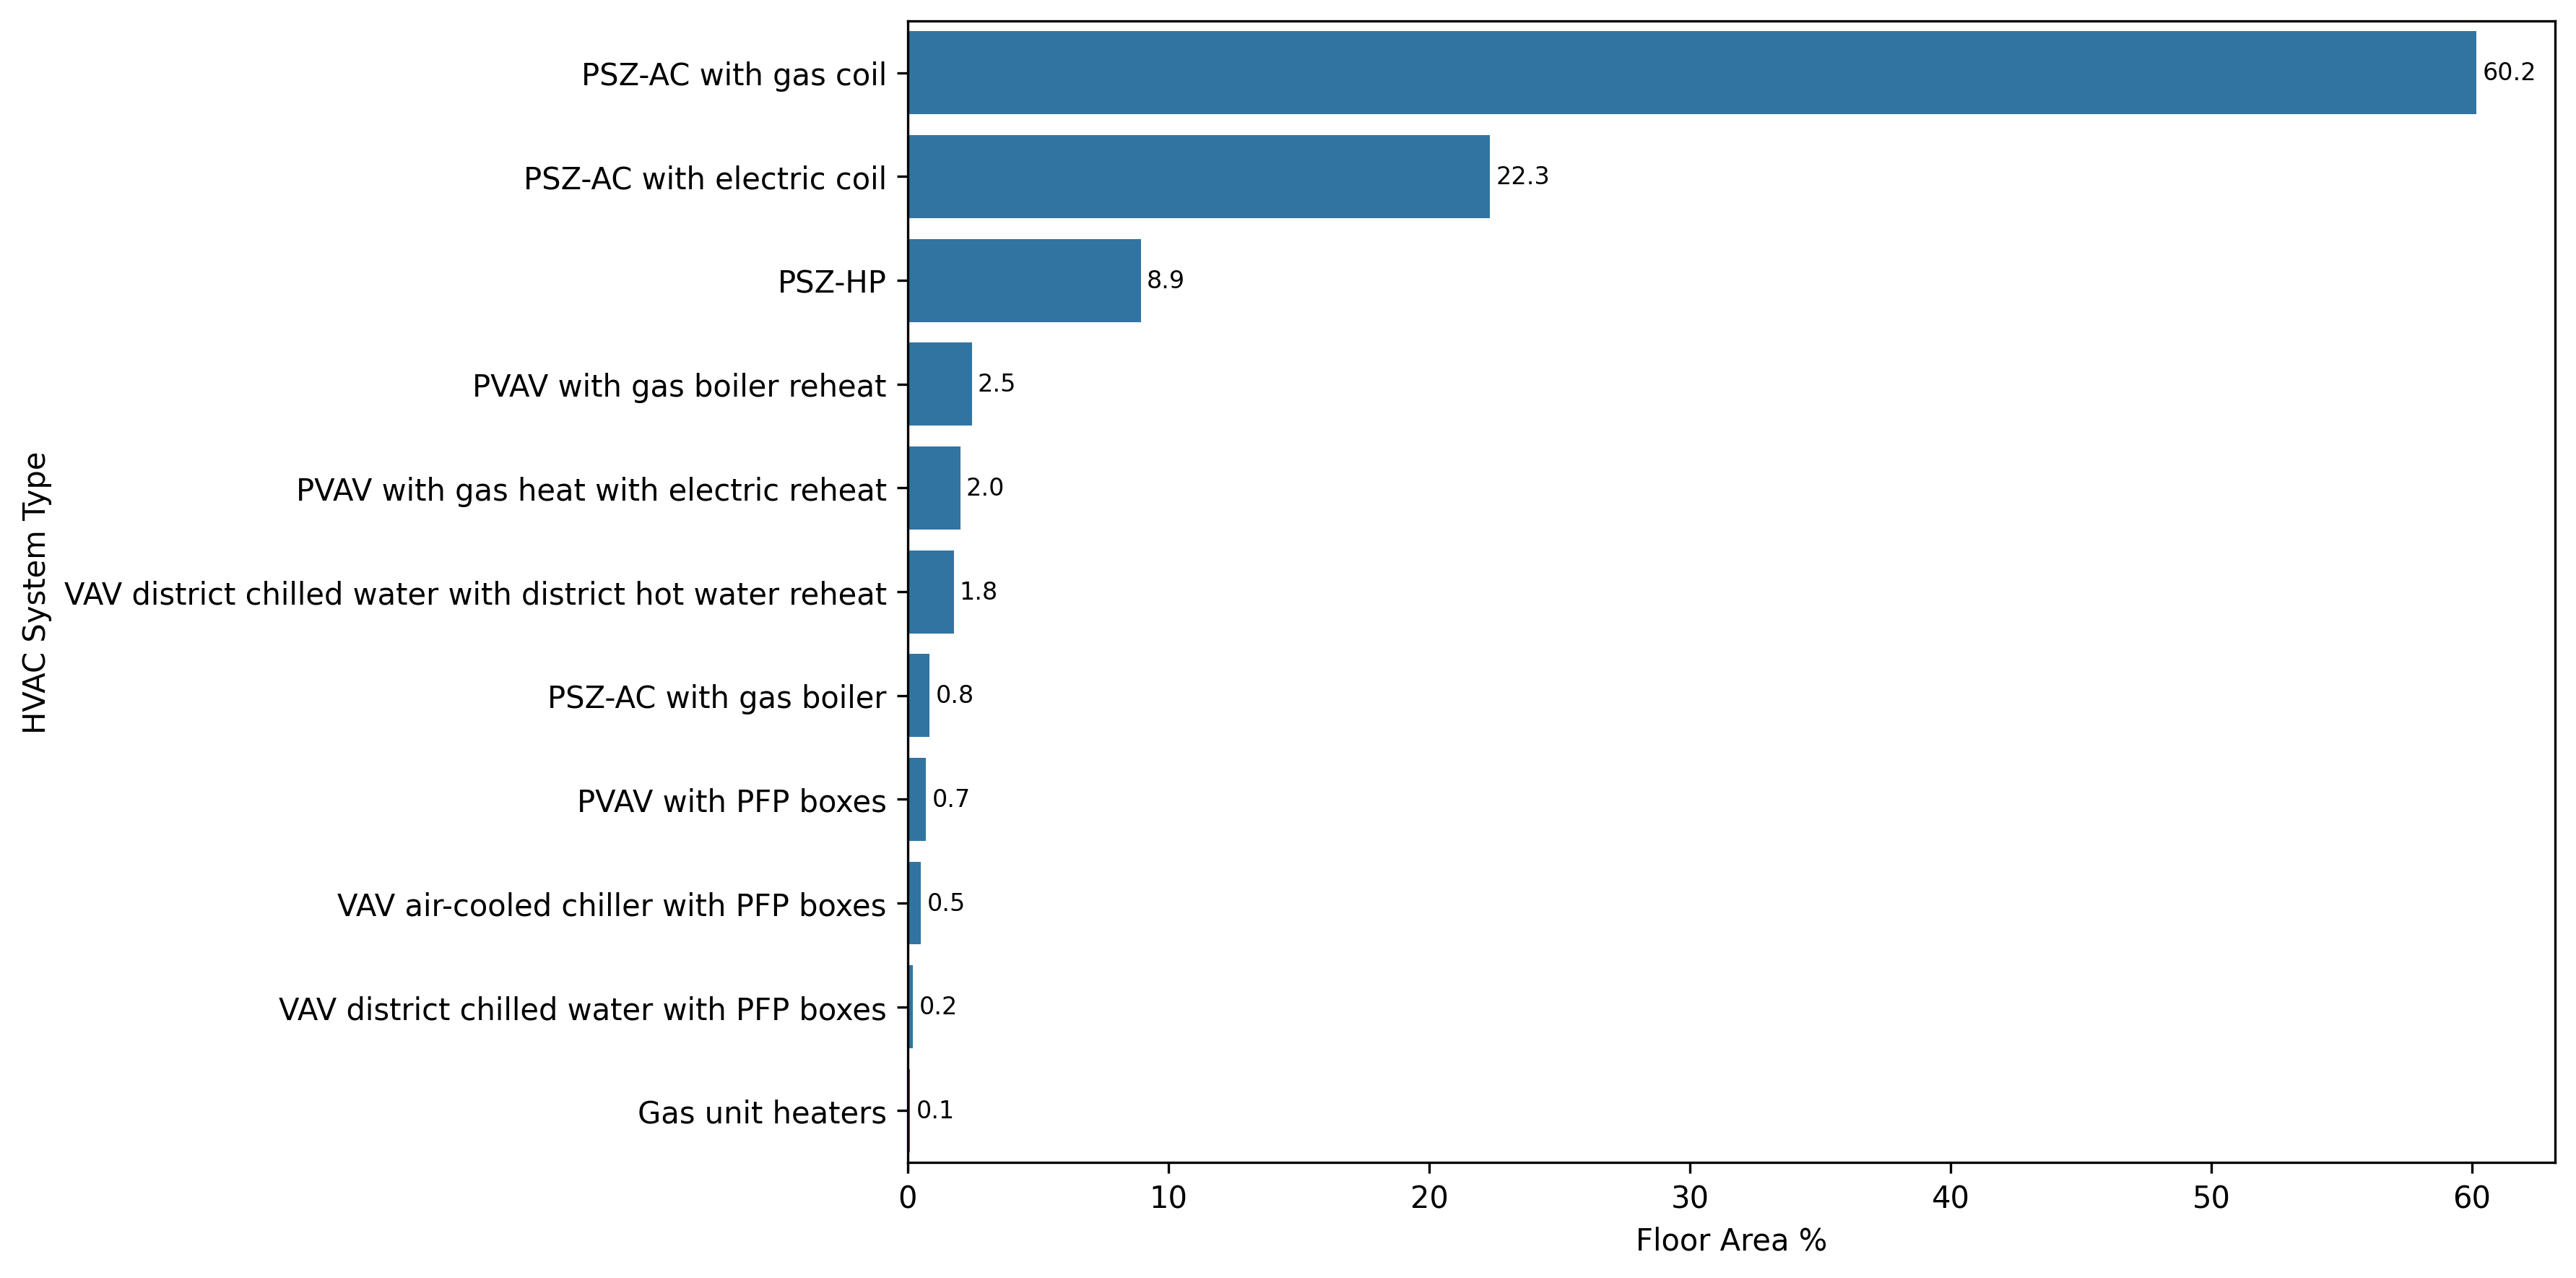
\includegraphics[width=1.0\textwidth]{figures/HVAC_SYS_Type_PREV_FSR.png}
    \caption[HVAC system type prevalence in full service restaurants]{Prevalence of ComStock HVAC system types by total stock floor area; full service restaurants.}
    \label{fig:hvac_sys_type_prevalence_fsr}
\end{figure}

\begin{figure}
    \centering 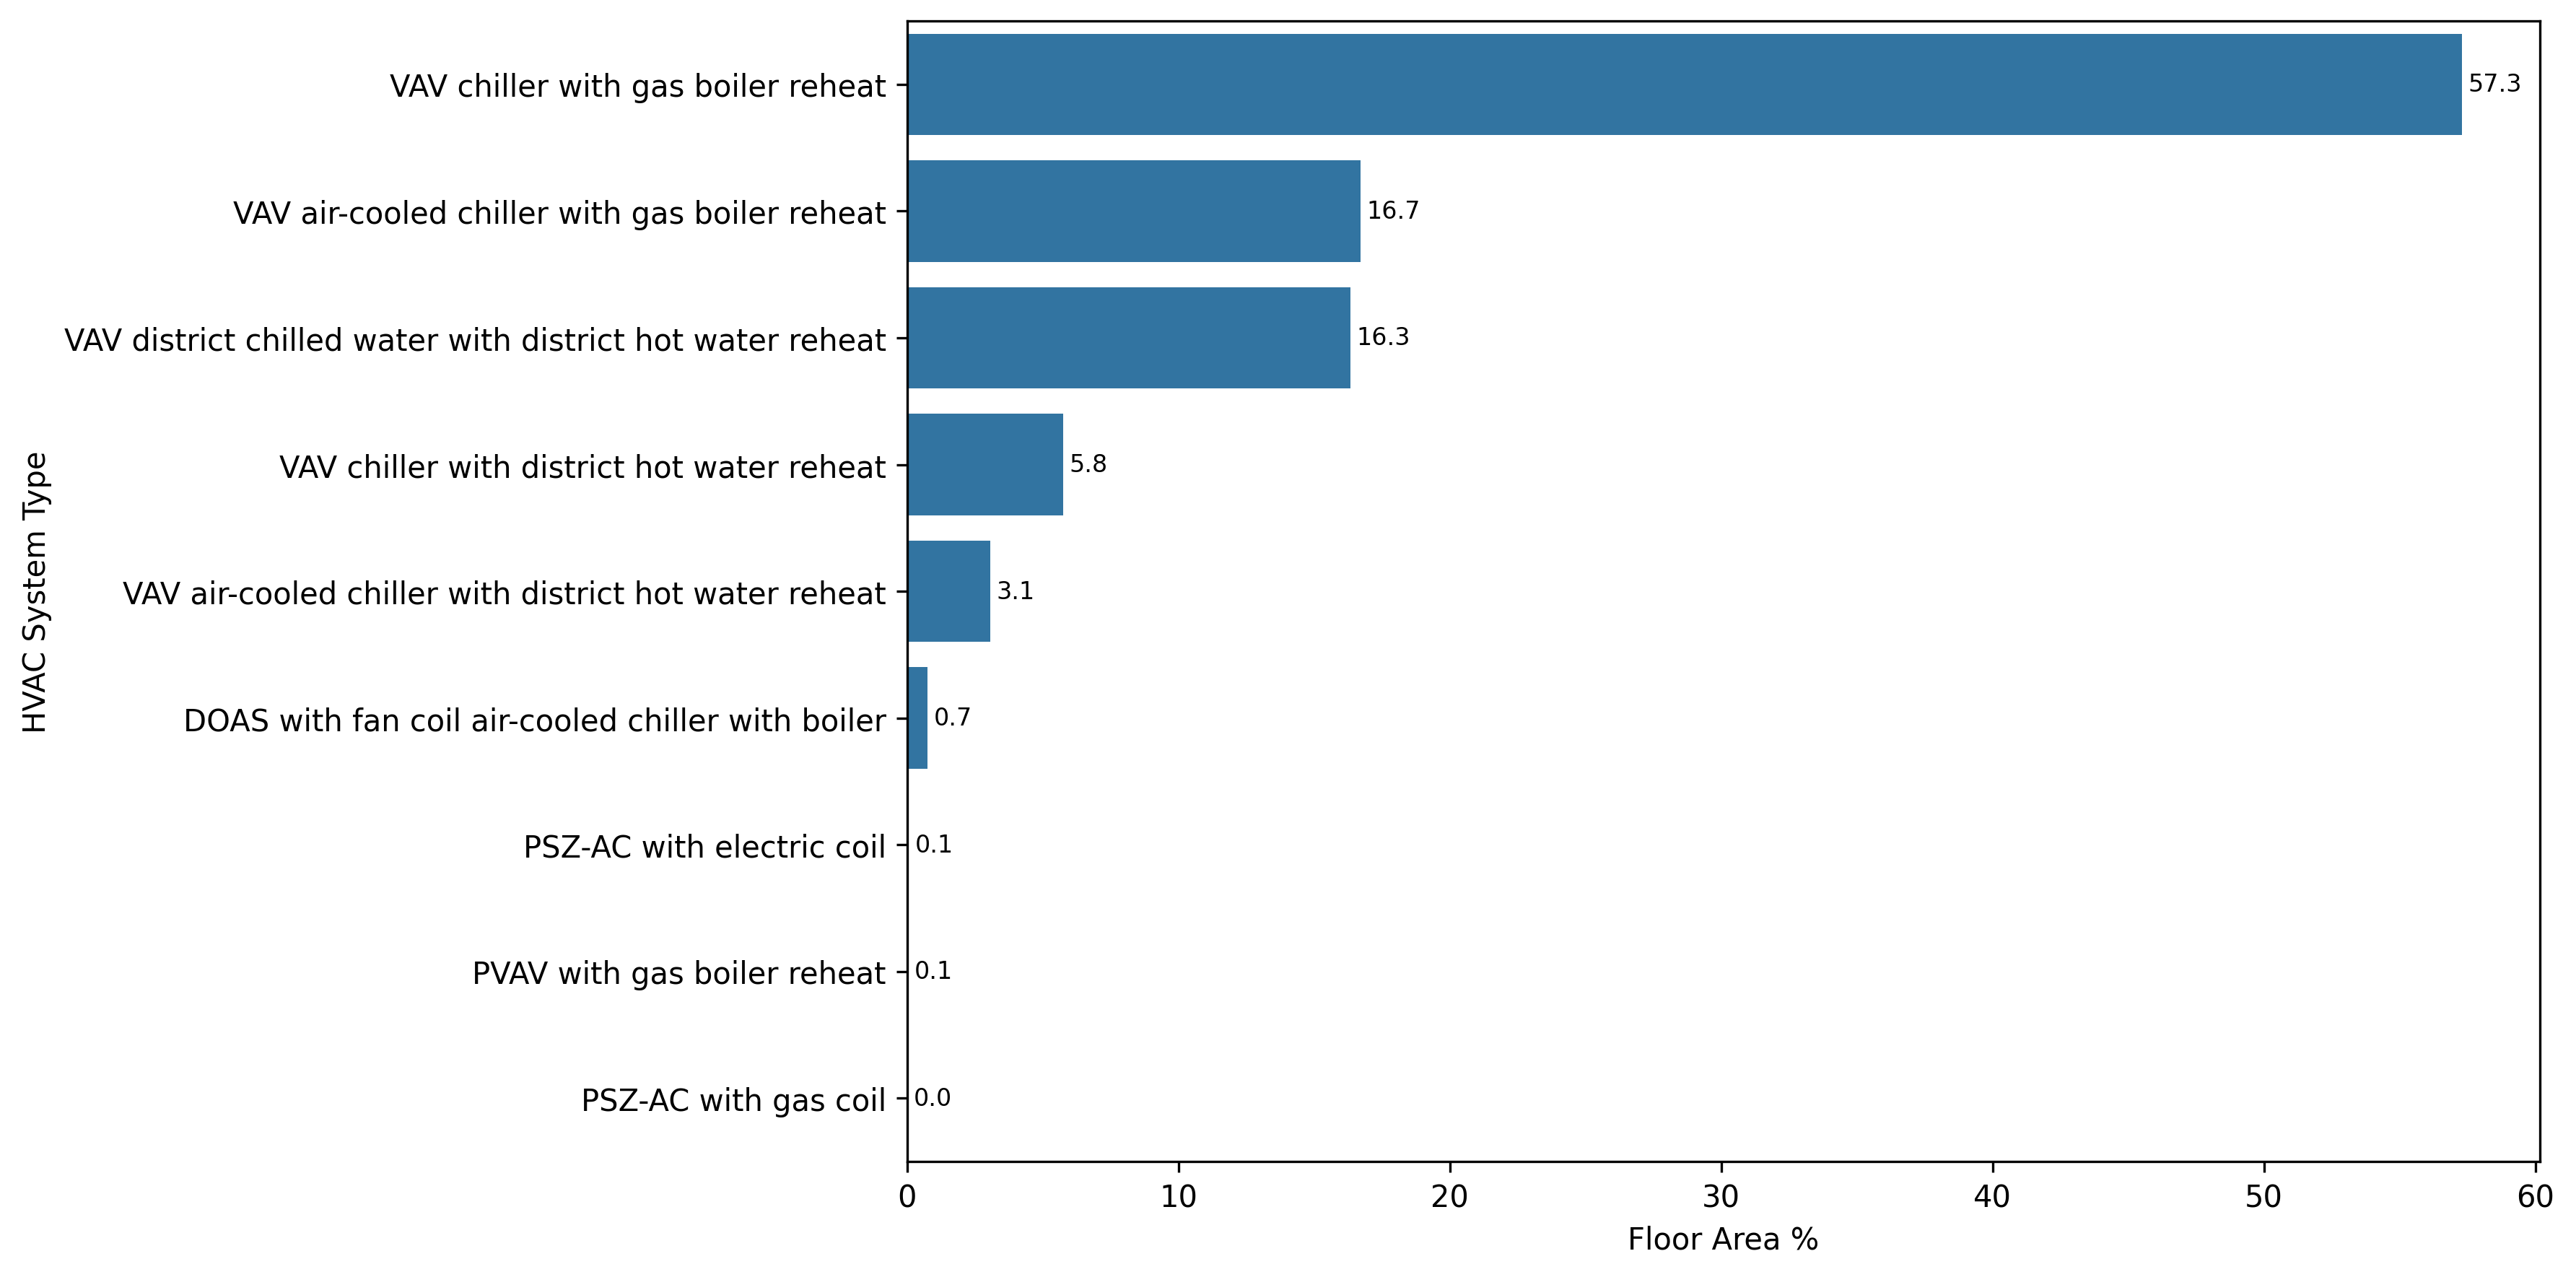
\includegraphics[width=1.0\textwidth]{figures/HVAC_SYS_Type_PREV_HOS.png}
    \caption[HVAC system type prevalence in hospitals]{Prevalence of ComStock HVAC system types by total stock floor area; hospitals.}
    \label{fig:hvac_sys_type_prevalence_hos}
\end{figure}

\begin{figure}
  \centering 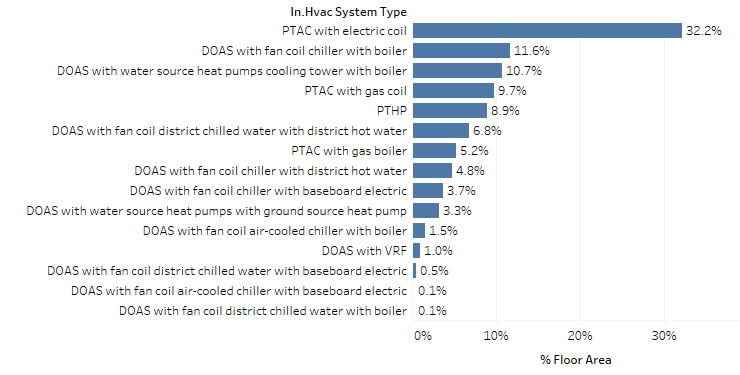
\includegraphics[width=1.0\textwidth]{figures/HVAC_SYS_Type_PREV_LrgHotel.png}
  \caption[HVAC system type prevalence in large hotels]{Prevalence of ComStock HVAC system types by total stock floor area; large hotels.}
  \label{fig:HVAC_SYS_Type_PREV_LrgHotel}
\end{figure}

\begin{figure}
    \centering 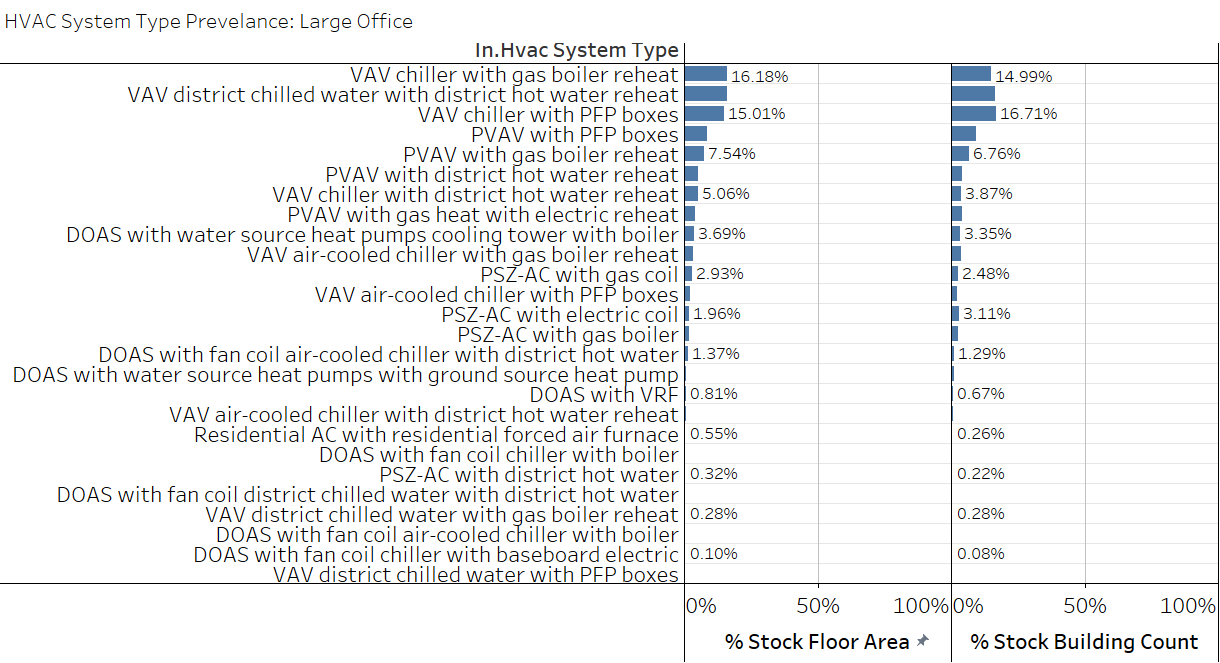
\includegraphics[width=1.0\textwidth]{figures/HVAC_SYS_Type_PREV_LrgOffice.png}
    \caption[HVAC system type prevalence in large offices]{Prevalence of ComStock HVAC system types by total stock floor area; large offices.}
    \label{fig:hvac_sys_type_prevalence_lrgoffice}
\end{figure}

\begin{figure}
    \centering 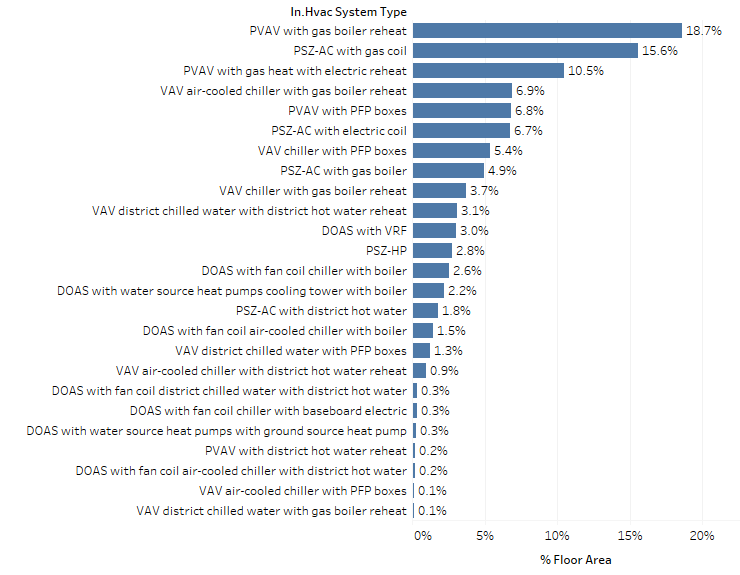
\includegraphics[width=1.0\textwidth]{figures/HVAC_SYS_Type_PREV_MedOffice.png}
    \caption[HVAC system type prevalence in medium offices]{Prevalence of ComStock HVAC system types by total stock floor area; medium offices.}
    \label{fig:hvac_sys_type_prevalence_medoffice}
\end{figure}

\begin{figure}
    \centering 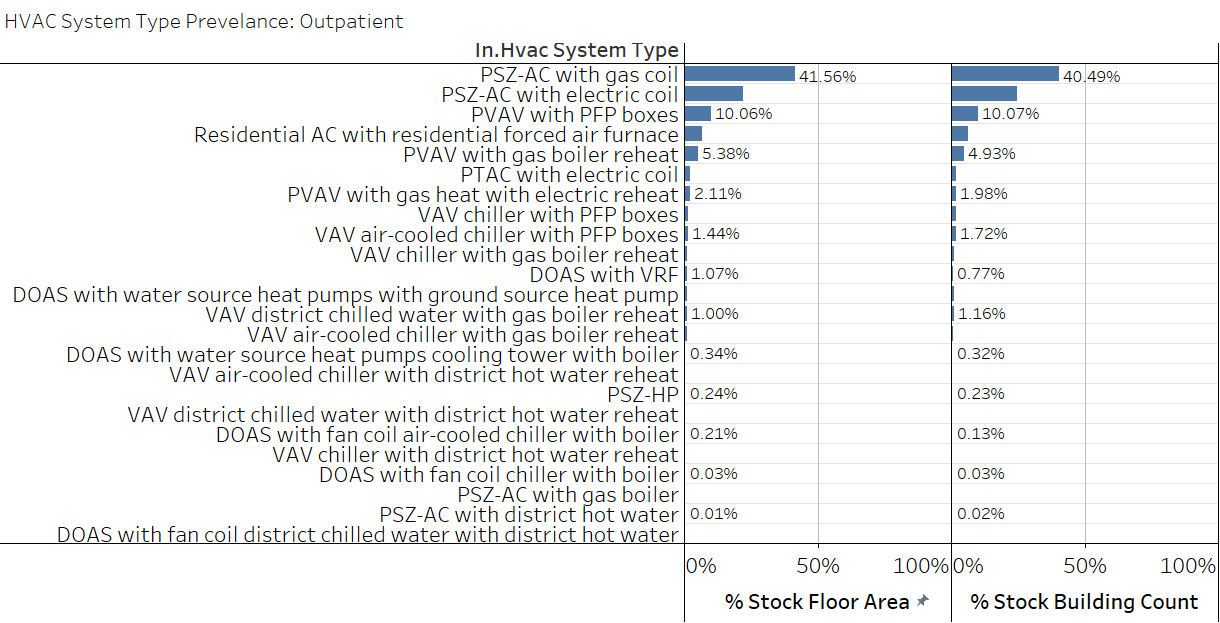
\includegraphics[width=1.0\textwidth]{figures/HVAC_SYS_Type_PREV_Outpatient.png}
    \caption[HVAC system type prevalence in outpatient]{Prevalence of ComStock HVAC system types by total stock floor area; outpatient.}
    \label{fig:hvac_sys_type_prevalence_outpatient}
\end{figure}

\begin{figure}
    \centering 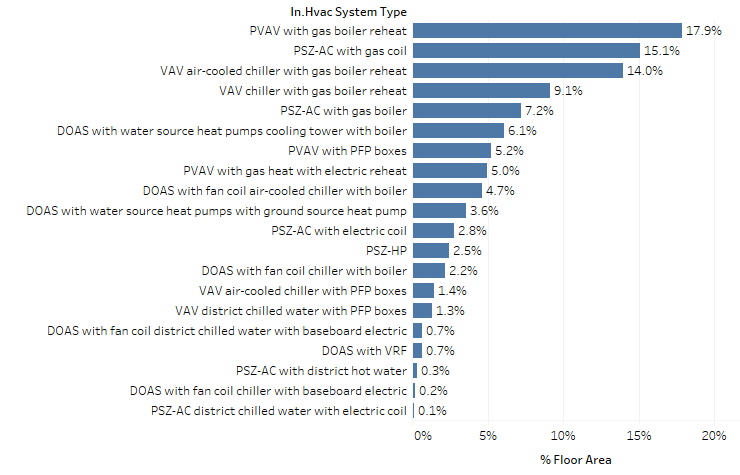
\includegraphics[width=1.0\textwidth]{figures/HVAC_SYS_Type_PREV_Primary_School.png}
    \caption[HVAC system type prevalence in primary schools]{Prevalence of ComStock HVAC system types by total stock floor area; primary schools.}
    \label{fig:hvac_sys_type_prevalence_primary_school}
\end{figure}

\begin{figure}
    \centering 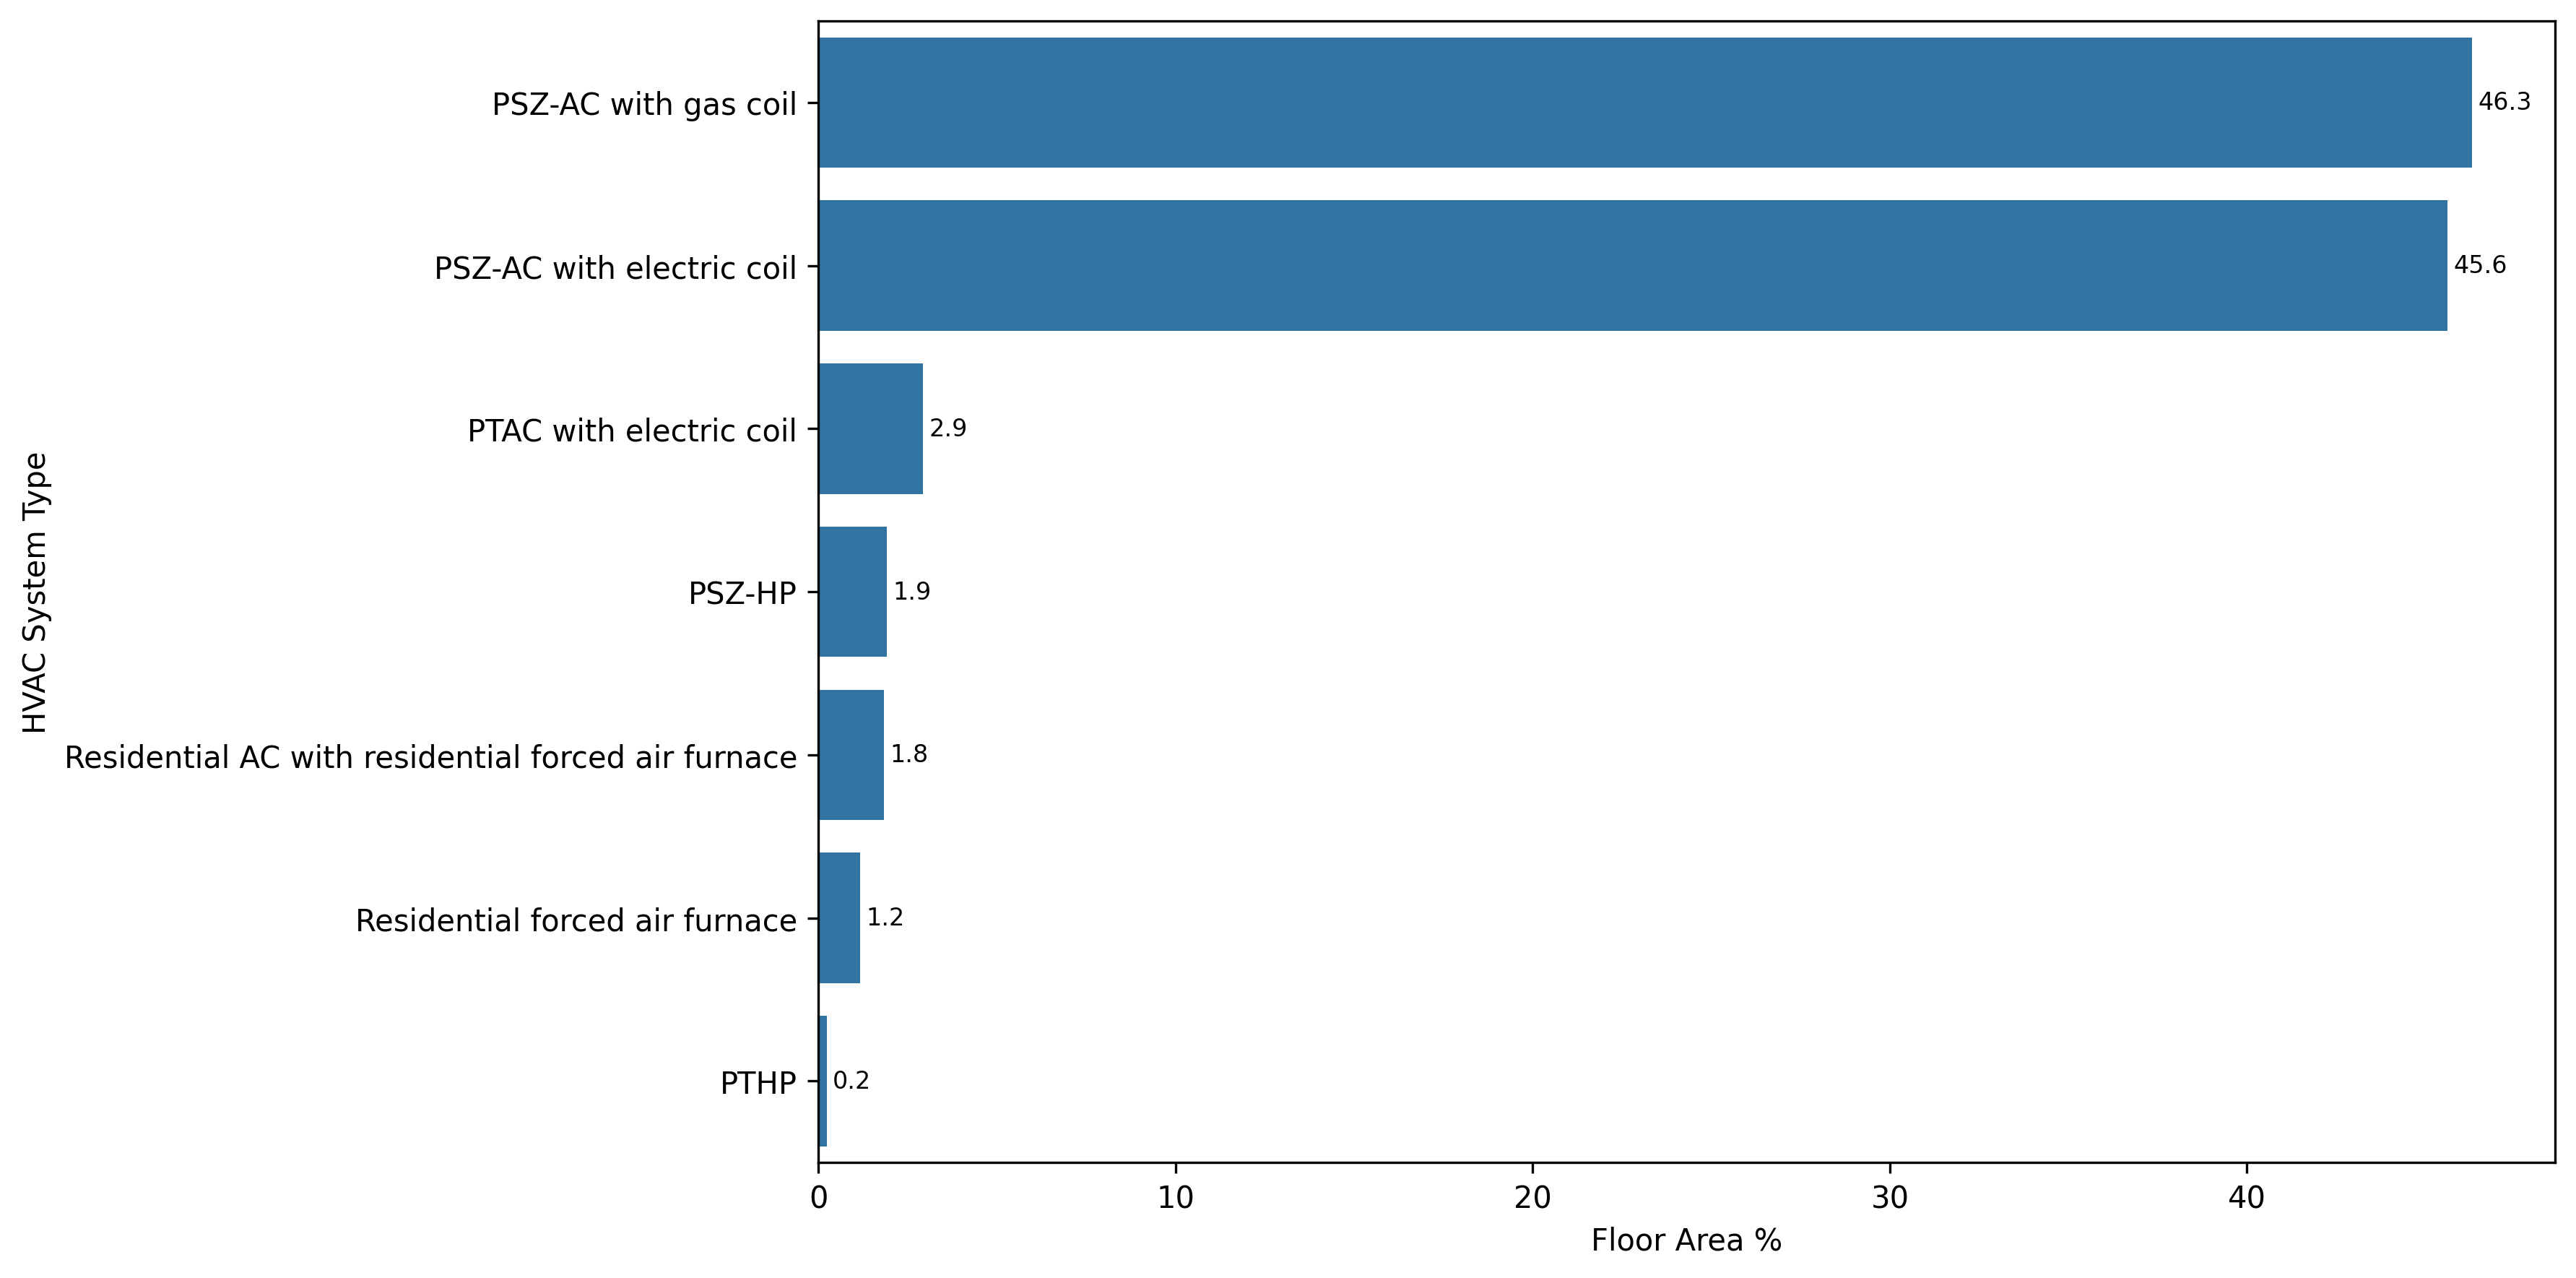
\includegraphics[width=1.0\textwidth]{figures/HVAC_SYS_Type_PREV_QSR.png}
    \caption[HVAC system type prevalence in quick service restaurants]{Prevalence of ComStock HVAC system types by total stock floor area; quick service restaurants.}
    \label{fig:hvac_sys_type_prevalence_qsr}
\end{figure}

\begin{figure}
    \centering 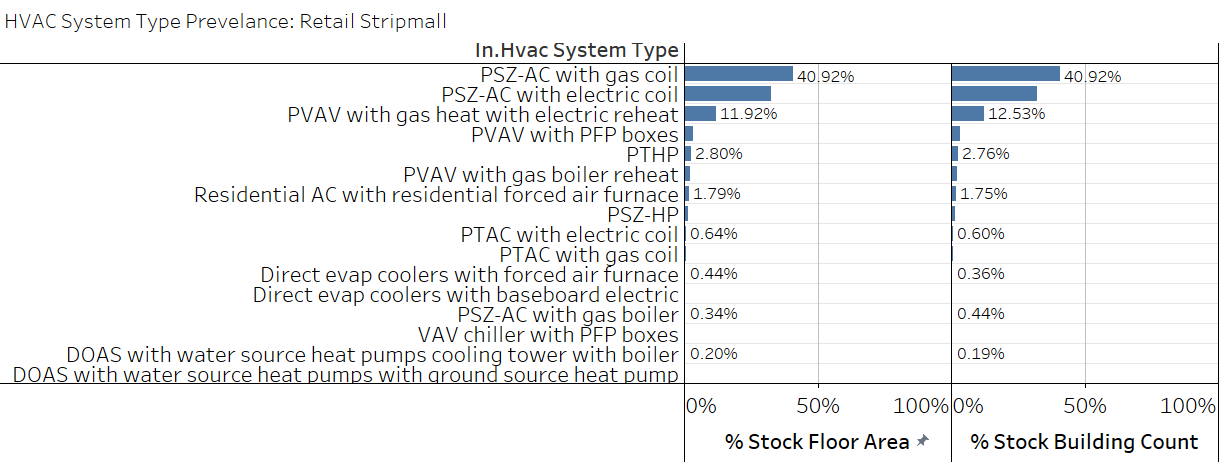
\includegraphics[width=1.0\textwidth]{figures/HVAC_SYS_Type_PREV_Retail_Stripmall.png}
    \caption[HVAC system type prevalence in strip malls]{Prevalence of ComStock HVAC system types by total stock floor area; strip malls.}
    \label{fig:hvac_sys_type_prevalence_retail_strip_mall}
\end{figure}

\begin{figure}
    \centering 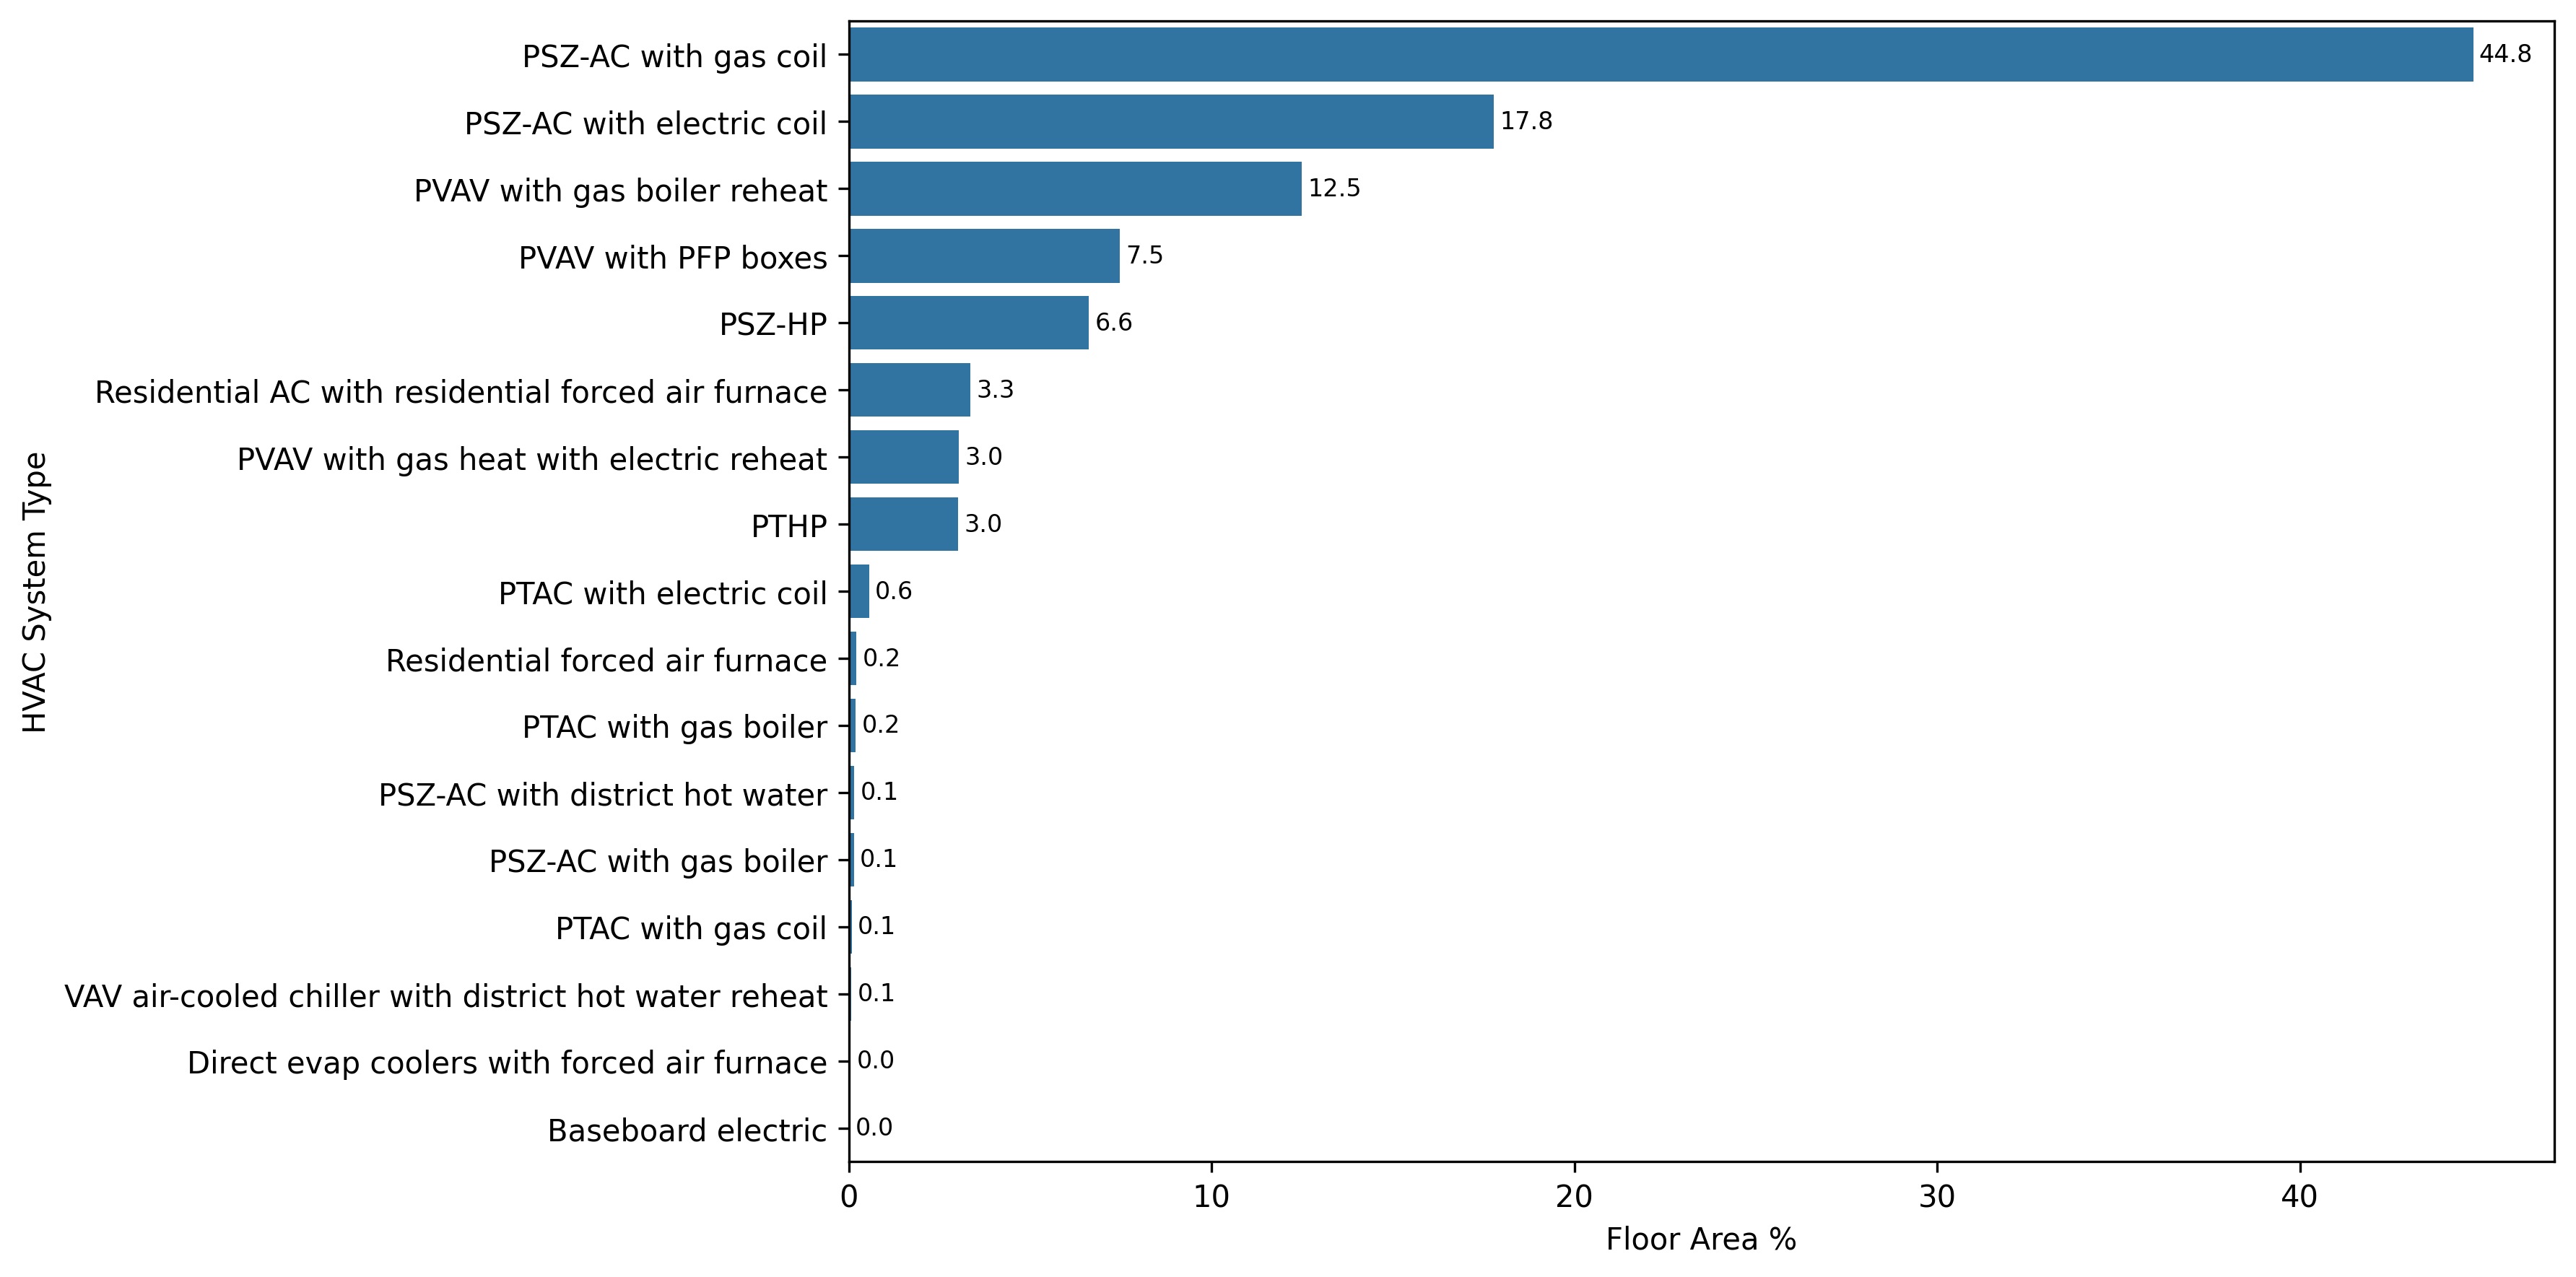
\includegraphics[width=1.0\textwidth]{figures/HVAC_SYS_Type_PREV_Retail.png}
    \caption[HVAC system type prevalence in retail]{Prevalence of ComStock HVAC system types by total stock floor area; retail.}
    \label{fig:hvac_sys_type_prevalence_retail}
\end{figure}

\begin{figure}
    \centering 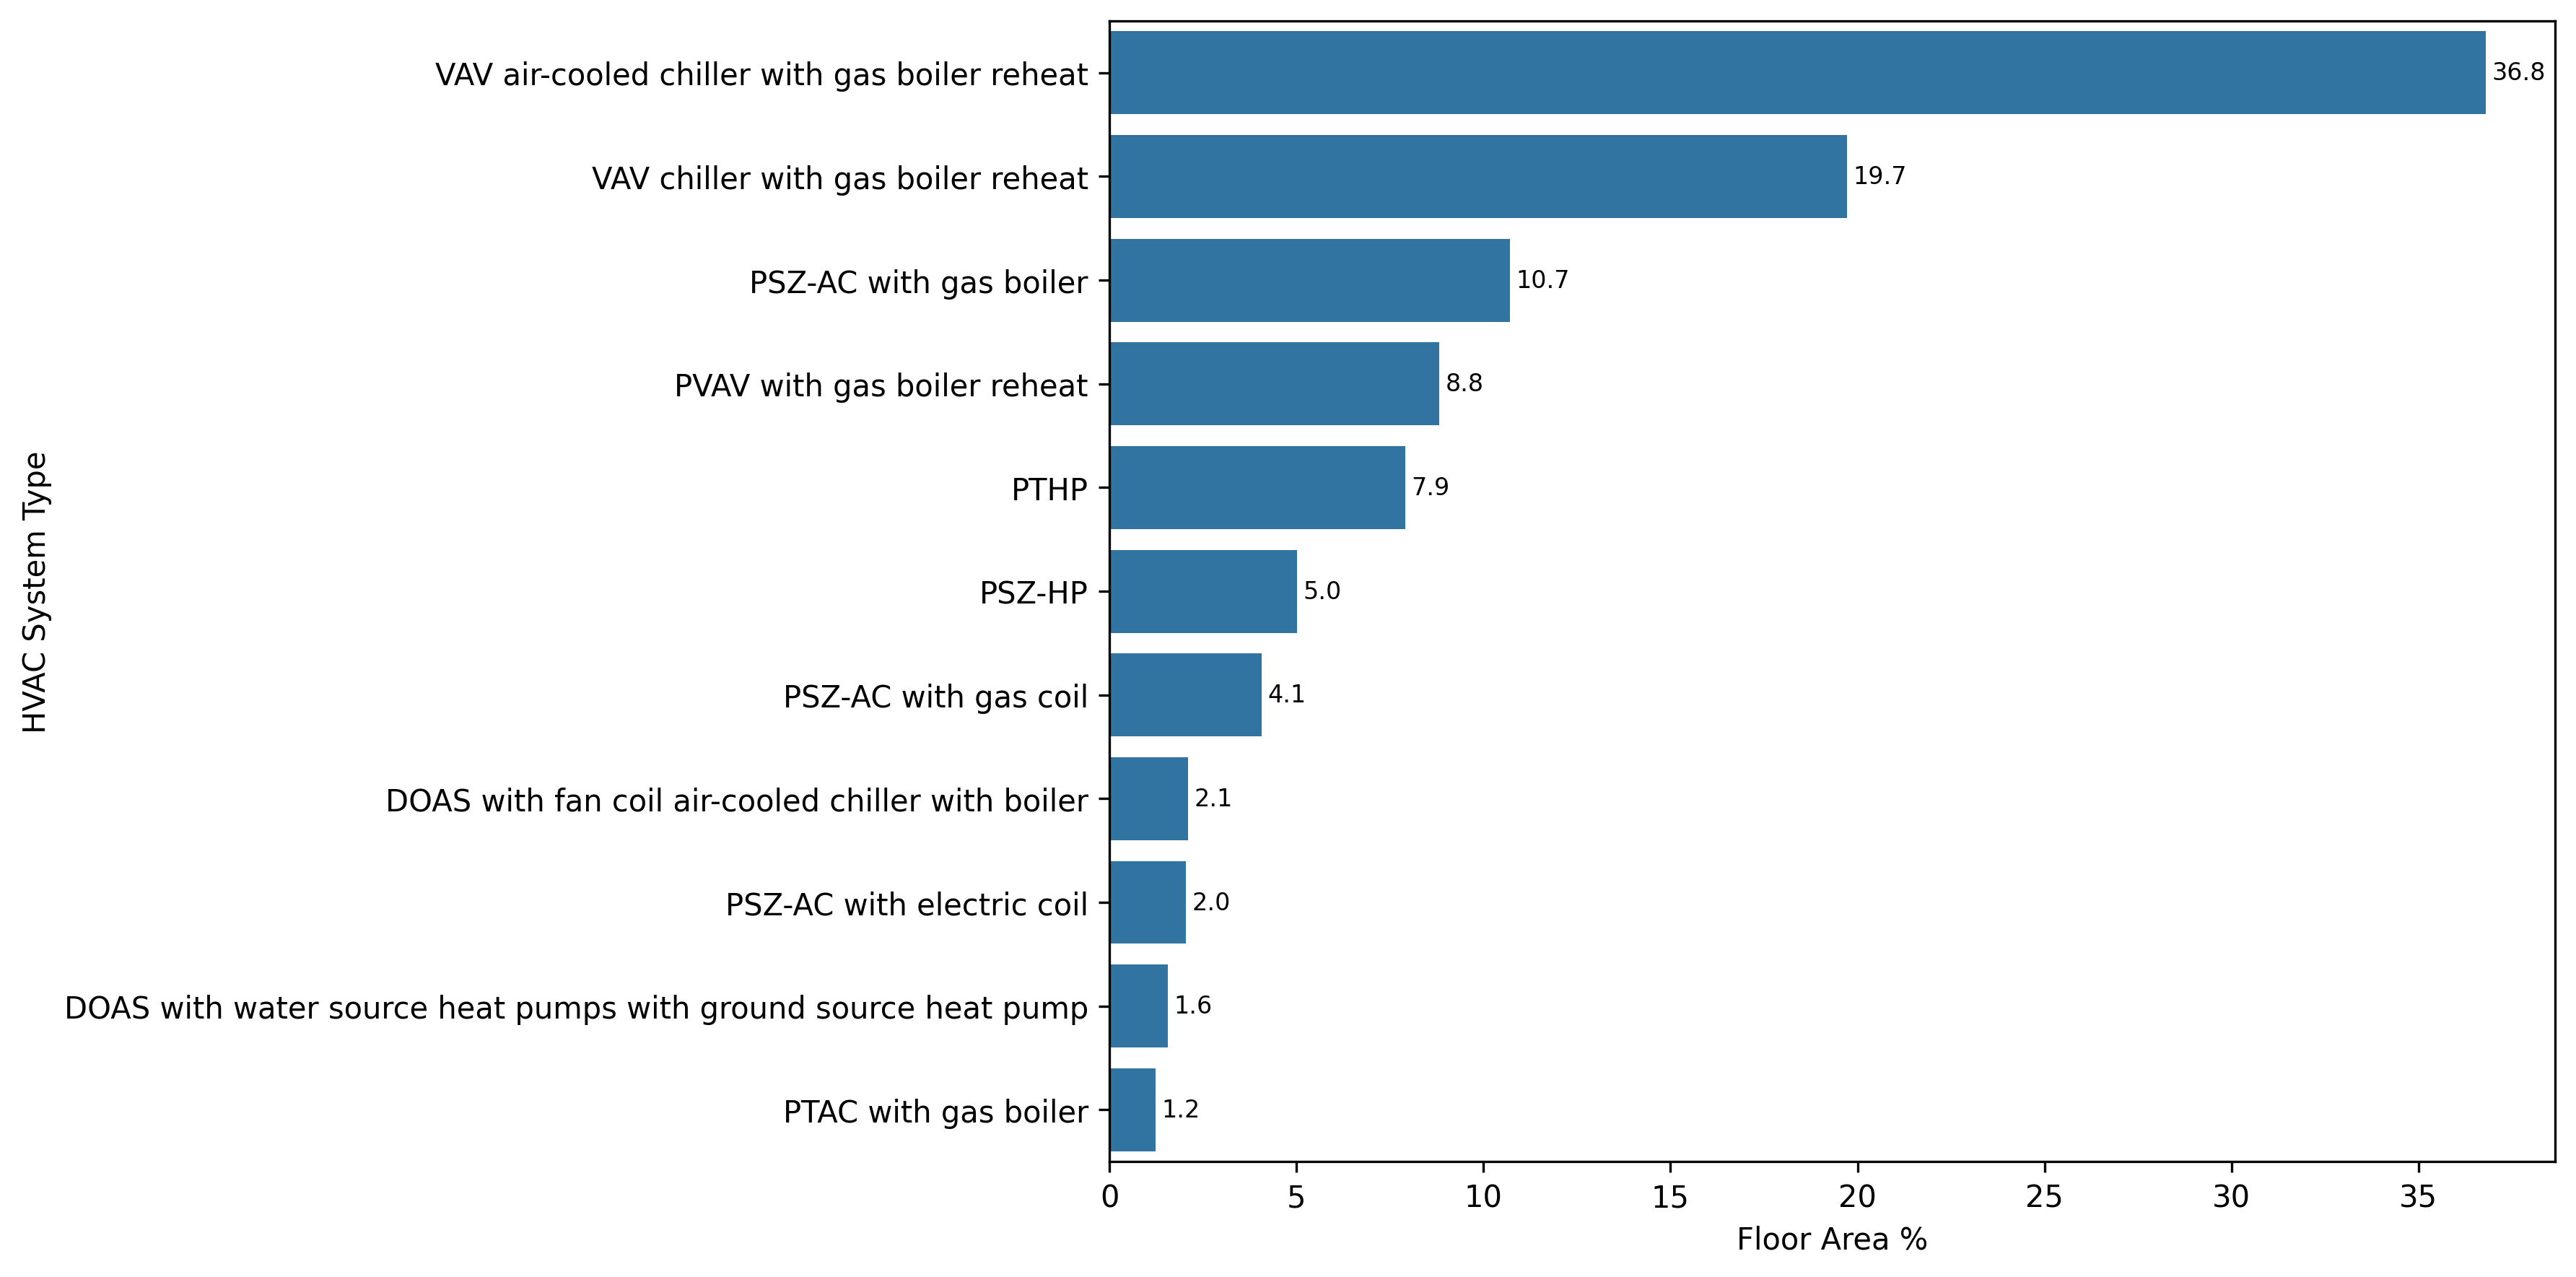
\includegraphics[width=1.0\textwidth]{figures/HVAC_SYS_Type_PREV_Secondary_School.png}
    \caption[HVAC system type prevalence in secondary schools]{Prevalence of ComStock HVAC system types by total stock floor area; secondary schools.}
    \label{fig:hvac_sys_type_prevalence_secondary_school}
\end{figure}

\begin{figure}
    \centering 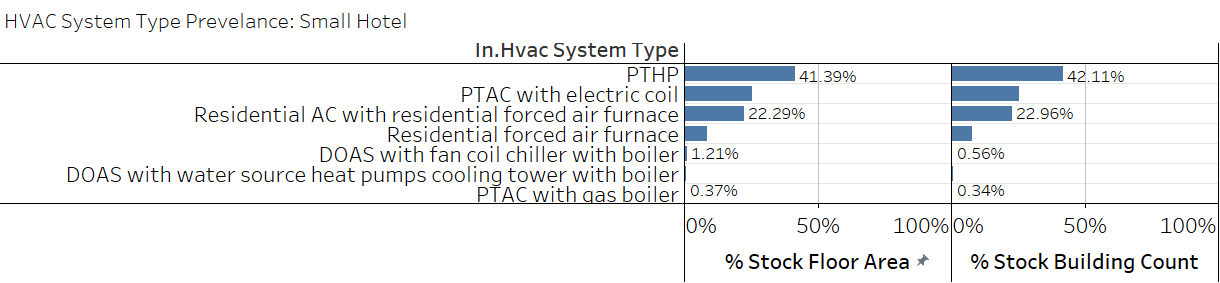
\includegraphics[width=1.0\textwidth]{figures/HVAC_SYS_Type_PREV_Small_Hotel.png}
    \caption[HVAC system type prevalence in small hotels]{Prevalence of ComStock HVAC system types by total stock floor area; small hotels.}
    \label{fig:hvac_sys_type_prevalence_small_hotel}
\end{figure}

\begin{figure}
    \centering 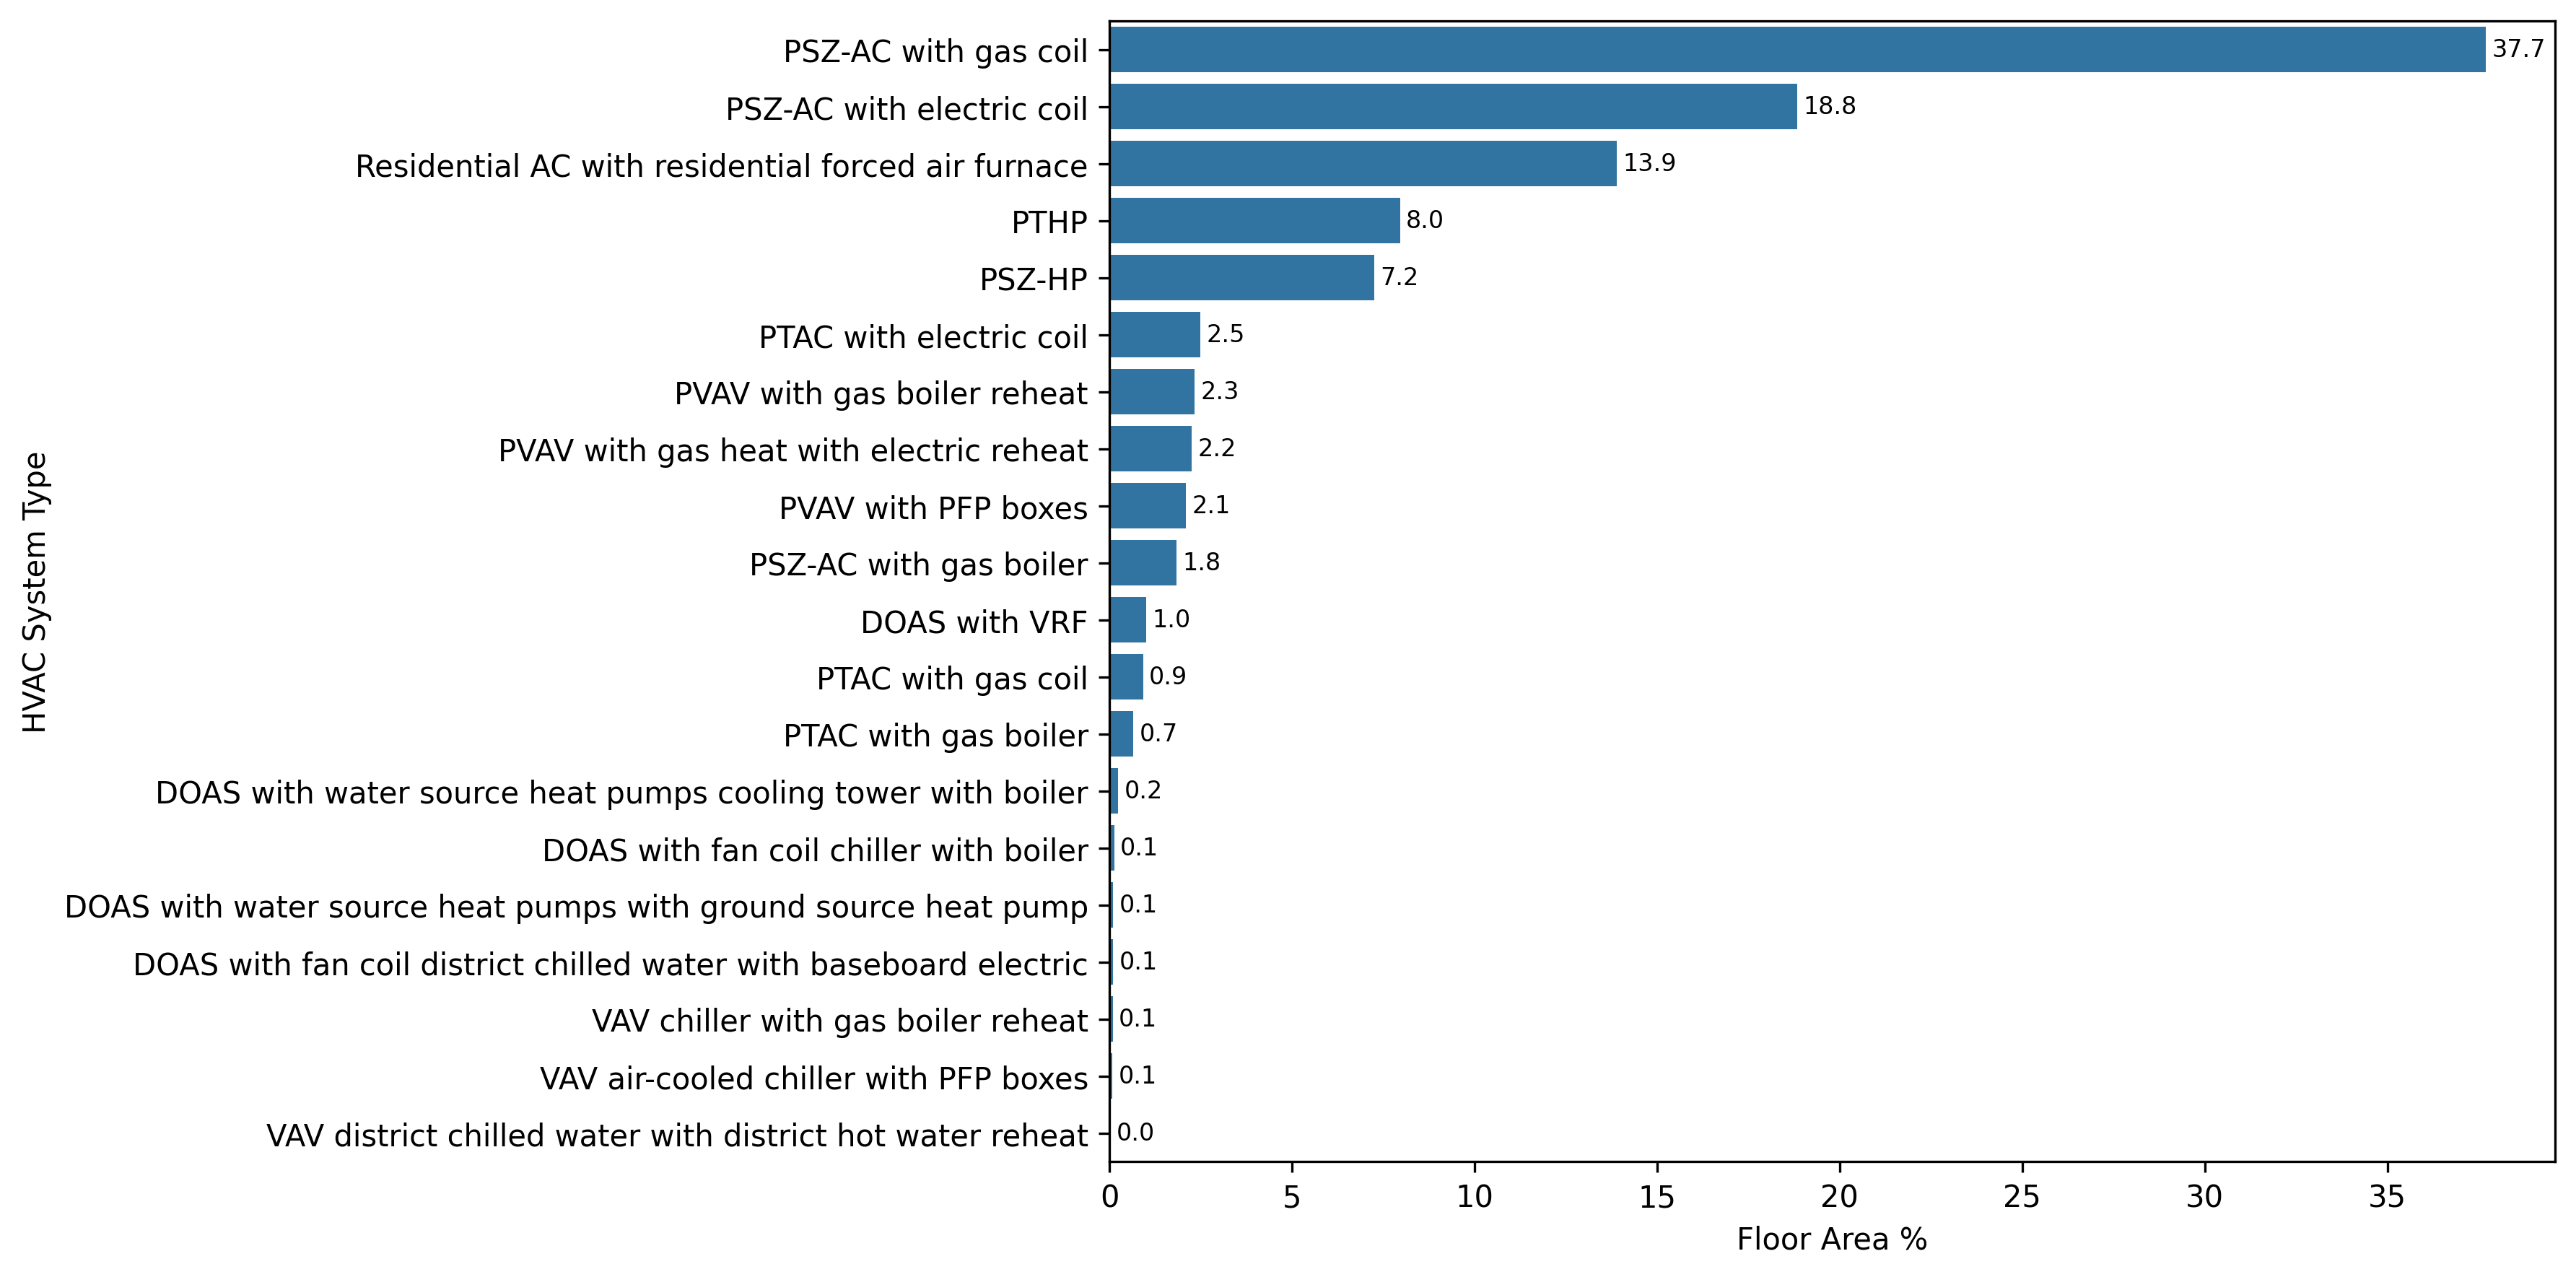
\includegraphics[width=1.0\textwidth]{figures/HVAC_SYS_Type_PREV_Small_Office.png}
    \caption[HVAC system type prevalence in small offices]{Prevalence of ComStock HVAC system types by total stock floor area; small offices.}
    \label{fig:hvac_sys_type_prevalence_small_office}
\end{figure}

\begin{figure}
    \centering 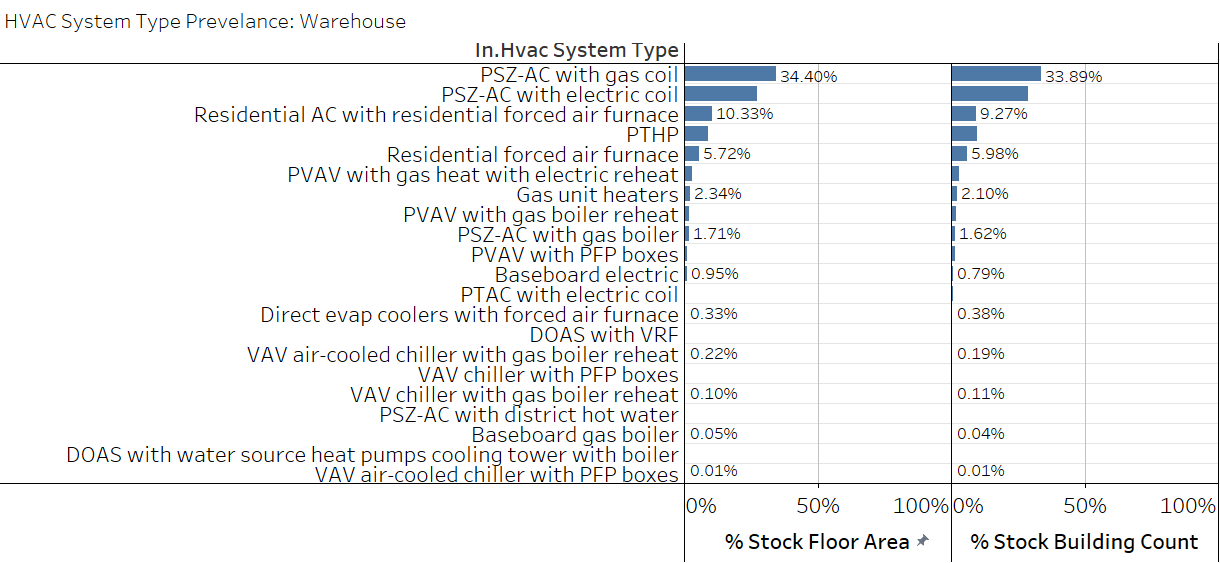
\includegraphics[width=1.0\textwidth]{figures/HVAC_SYS_Type_PREV_Warehouse.png}
    \caption[HVAC system type prevalence in warehouses]{Prevalence of ComStock HVAC system types by total stock floor area; warehouses.}
    \label{fig:hvac_sys_type_prevalence_warehouse}
\end{figure}

\begin{figure}
    \centering 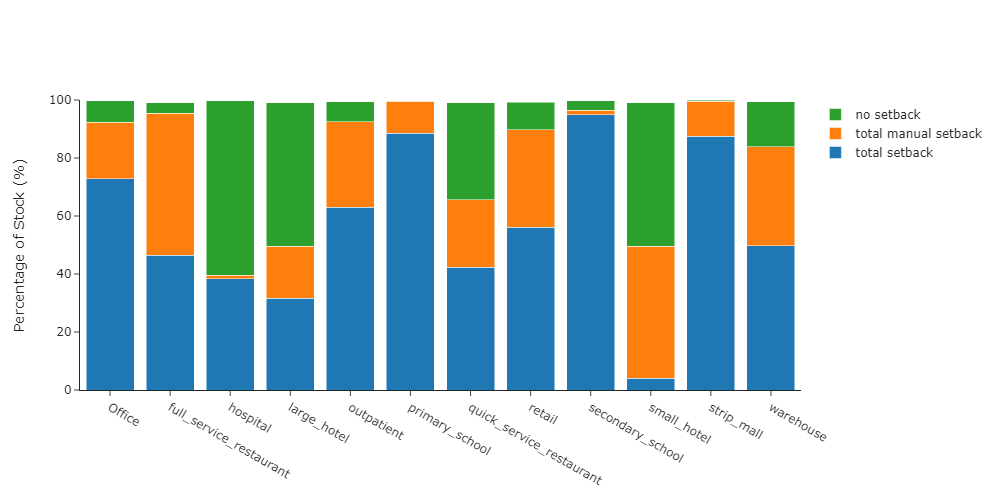
\includegraphics[width=1.0\textwidth]{figures/cbecs_therm_summary.png}
    \caption[Percentage of buildings with thermostat setbacks from the CBECS 2012 survey]{Percentage of buildings with thermostat setbacks by building type from the CBECS 2012 survey.}
    \label{fig:cbecs_therm_setback_summary}
\end{figure}

\begin{figure}
    \centering \includegraphics[width=1.0\textwidth]{figures/All_Building_Types_thermostat_scatter.png}
    \caption[Correlation between thermostat set point and thermostat setback from BAS data]{Thermostat heating and cooling set point-setback delta correlation from BAS data sources; all building types.}
    \label{fig:therm_setpoint_setback}
\end{figure}

\pagebreak

\begin{figure}
    \centering 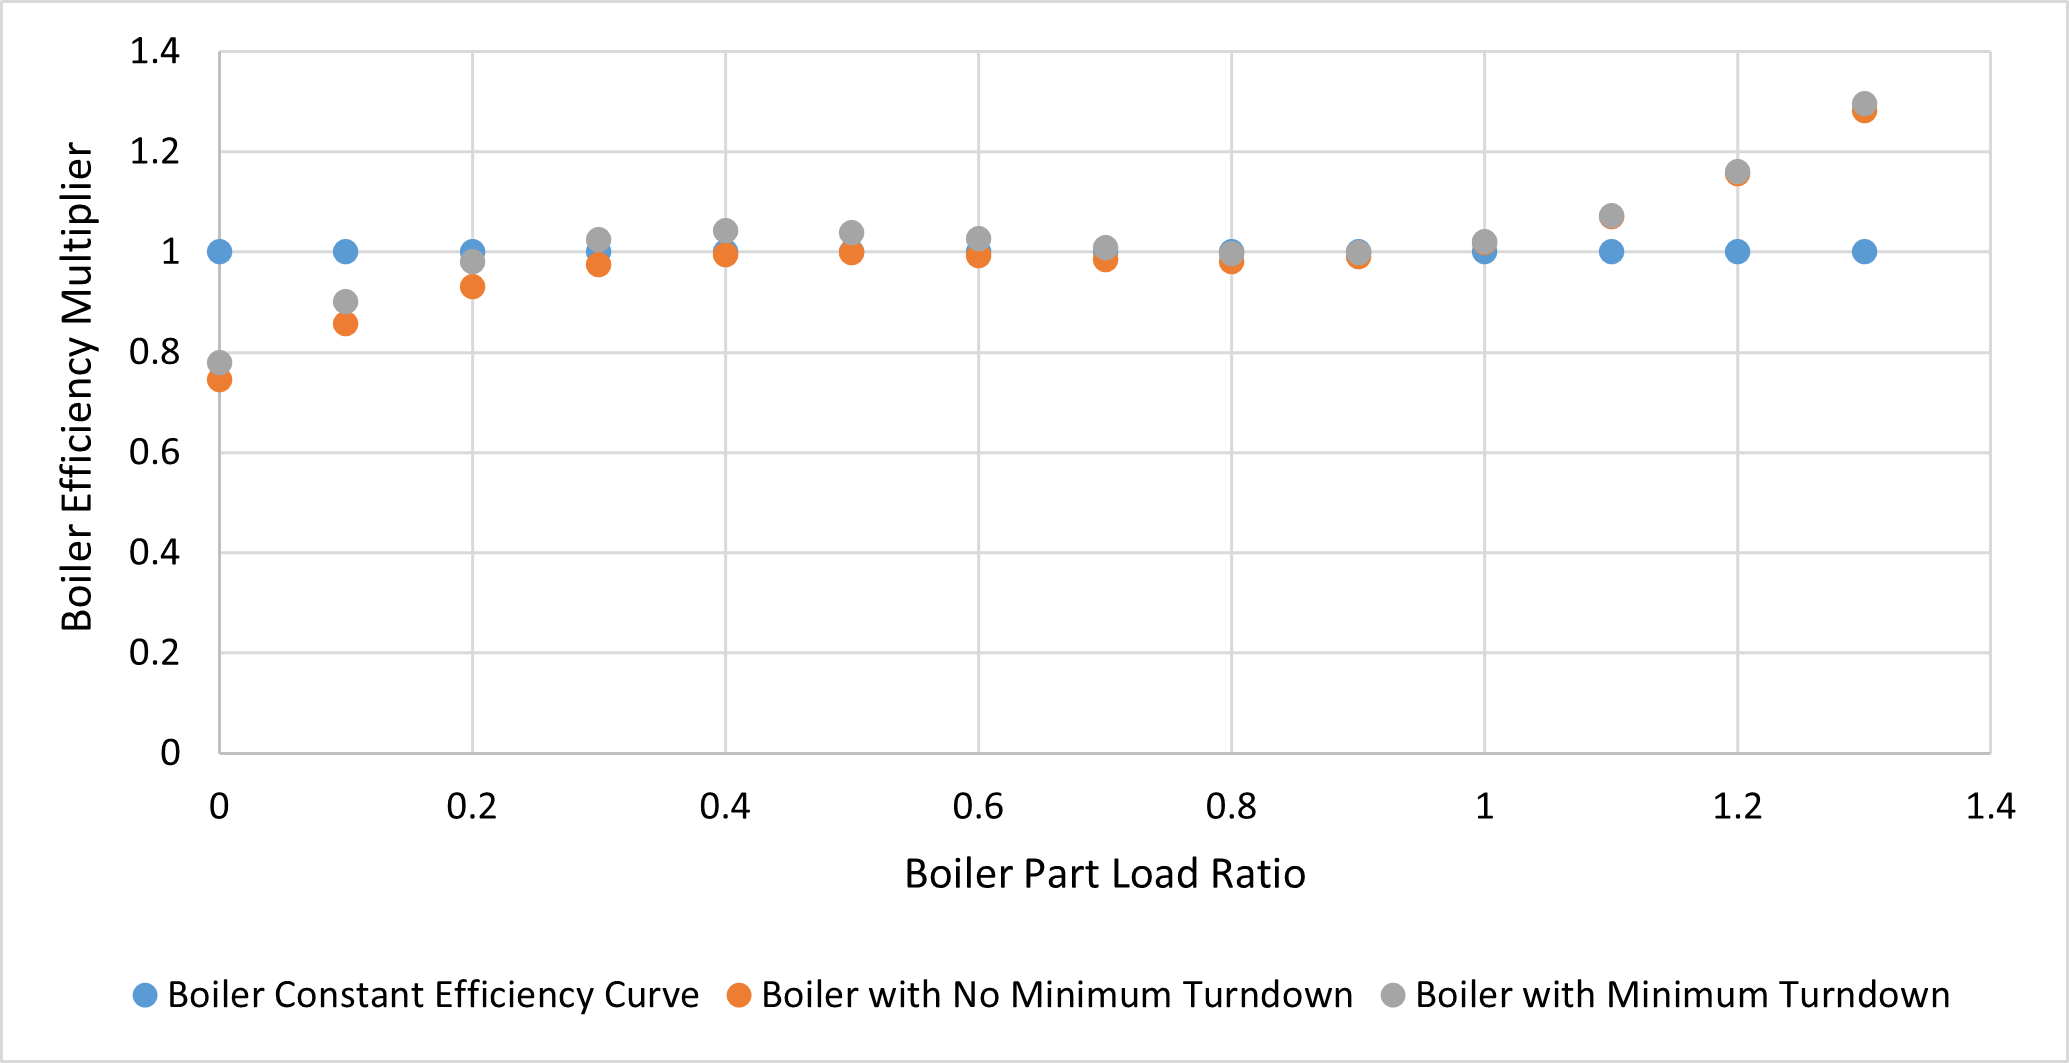
\includegraphics[width=1.0\textwidth]{figures/boiler_performance_curves.png}
    \caption[Boiler part load performance curves]{Boiler part load performance curves.}
    \label{fig:blr_plr_curves}
\end{figure}


\begin{figure}
    \centering \includegraphics[width=1.0\textwidth]{figures/EIRFPLR.png}
    \caption[DX cooling energy input ratio as a function of part load ratio performance curves]{DX cooling energy input ratio as a function of part load ratio performance curves.}
    \label{fig:dx_eirfplr}
\end{figure}

\begin{figure}
    \centering \includegraphics[width=1.0\textwidth]{figures/CAPFF.png}
    \caption[DX cooling capacity as a function of airflow performance curves]{DX cooling capacity as a function of airflow performance curves.}
    \label{fig:dx_capff}
\end{figure}

\begin{figure}
    \centering \includegraphics[width=1.0\textwidth]{figures/EIRFF.png}
    \caption[DX cooling energy input ratio as a function of airflow performance curves]{DX cooling energy input ratio as a function of airflow performance curves.}
    \label{fig:dx_eirff}
\end{figure}

\begin{figure}
    \centering \includegraphics[width=1.0\textwidth]{figures/EIRFT.png}
    \caption[DX cooling energy input ratio as a function of temperature performance curves]{DX cooling energy input ratio as a function of temperature performance curves. Independent variables are outdoor air dry bulb temperature (y-axis, degrees Celsius) and wet bulb temperature entering the cooling coil (x-axis, degrees Celsius).}
    \label{fig:dx_eirft}
\end{figure}

\begin{figure}
    \centering \includegraphics[width=1.0\textwidth]{figures/CAPFT.png}
    \caption[DX cooling capacity as a function of temperature performance curves]{DX cooling capacity as a function of temperature performance curves. Independent variables are outdoor air dry bulb temperature (y-axis, degrees Celsius) and wet bulb temperature entering the cooling coil (x-axis, degrees Celsius).}
    \label{fig:dx_capft}
\end{figure}

\begin{figure}
    \centering \includegraphics[width=1.0\textwidth]{figures/ashp_eirft.png}
    \caption[Air-source heat pump COP ratio as a function of outdoor air dry bulb temperature]{Air-source heat pump COP ratio as a function of outdoor air dry bulb temperature.}
    \label{fig:ashp_eirft}
\end{figure}

\begin{figure}
    \centering \includegraphics[width=1.0\textwidth]{figures/ashp_eirfplr.png}
    \caption[Air-source heat pump EIR ratio as a function of part load ratio]{Air-source heat pump EIR ratio as a function of part load ratio.}
    \label{fig:ashp_eirfplr}
\end{figure}

\begin{figure}
    \centering \includegraphics[width=1.0\textwidth]{figures/ashp_eirff.png}
    \caption[Air-source heat pump EIR ratio as a function of airflow fraction]{Air-source heat pump EIR ratio as a function of airflow fraction.}
    \label{fig:ashp_eirff}
\end{figure}

\begin{figure}
    \centering \includegraphics[width=1.0\textwidth]{figures/ashp_capft.png}
    \caption[Air-source heat pump capacity as a function of outdoor air dry bulb temperature]{Air-source heat pump capacity as a function of outdoor air dry bulb temperature.}
    \label{fig:ashp_capft}
\end{figure}

\begin{figure}
    \centering \includegraphics[width=1.0\textwidth]{figures/ashp_capff.png}
    \caption[Air-source heat pump capacity as a function of airflow ratio]{Air-source heat pump capacity as a function of airflow ratio.}
    \label{fig:ashp_capff}
\end{figure}

\begin{figure}
    \centering \includegraphics[width=1.0\textwidth]{figures/ac_chiller_eir_curves.png}
    \caption[Air-cooled chiller EIR as a function of part load ratio performance curves]{Air-cooled chiller EIR as a function of part load ratio performance curves. Independent variables beyond the curve limits will use the bound of the curve limit during simulation.}
    \label{fig:acc_eir_curves}
\end{figure}

\begin{figure}
    \centering \includegraphics[width=1.0\textwidth]{figures/AirCooled_Chiller_2010_PathA_Modifiers.png}
    \caption["AirCooledChiller2010PathA" modifier performance curves]{``AirCooledChiller2010PathA'' modifier performance curves; capacity as a function of temperature and EIR as a function of temperature. Independent variables beyond the curve limits will use the bound of the curve limit during simulation.}
    \label{fig:AirCooledChiller2010PathA_funct_curves}
\end{figure}

\begin{figure}
    \centering \includegraphics[width=1.0\textwidth]{figures/ChlrAirRecipQRatio_Modifiers.png}
    \caption["ChlrAirRecip" modifier performance curves]{``ChlrAirRecip'' modifier performance curves; capacity as a function of temperature and EIR as a function of temperature. Independent variables beyond the curve limits will use the bound of the curve limit during simulation.}
    \label{fig:ChlrAirRecipQRatio_curves}
\end{figure}

\begin{figure}
    \centering \includegraphics[width=1.0\textwidth]{figures/wcc_plr.png}
    \caption{Energy input ratio modifier as a function of water-cooled chiller part load ratio.}
    \label{fig:wcc_plr}
\end{figure}

\begin{figure}
    \centering \includegraphics[width=1.0\textwidth]{figures/WaterCooled_PositiveDisplacement_Chiller_LT150_2010_Modifiers.png}
    \caption[Performance curves for WCC]{Performance curves for ``WaterCooled PositiveDisplacement Chiller LT150 2010 Modifiers'' WCC.}
    \label{fig:wcc_WaterCooled_PositiveDisplacement_Chiller_LT150_2010_Modifiers}
\end{figure}

\begin{figure}
    \centering \includegraphics[width=1.0\textwidth]{figures/ChlrWtrPosDispPathAAll_Modifiers.png}
    \caption{Performance curves for ``ChlrWtrPosDispPathAAll Modifiers'' WCC.}
    \label{fig:wcc_ChlrWtrPosDispPathAAll_Modifiers}
\end{figure}

\begin{figure}
    \centering \includegraphics[width=1.0\textwidth]{figures/ground_loop_outlet_temperatures.png}
    \caption{Ground loop outlet vs. inlet temperature relationship for GSHPs.}
    \label{fig:gshp_loop_temps}
\end{figure}


\begin{figure}
    \centering \includegraphics[width=1.0\textwidth]{figures/refrigeration_MTold.png}
    \caption[Compressor performance for small, old, medium temperature compressors]{Power and capacity values as a function of suction and discharge temperature for small, old, medium-temperature compressors.}
    \label{fig:refrig_mt_old}
\end{figure}

\begin{figure}
    \centering \includegraphics[width=1.0\textwidth]{figures/refrigeration_MTnew.png}
    \caption[Compressor performance for large, new, medium temperature compressors]{Power and capacity values as a function of suction and discharge temperature for large, new, medium-temperature compressors.}
    \label{fig:refrig_mt_new}
\end{figure}

\begin{figure}
    \centering \includegraphics[width=1.0\textwidth]{figures/refrigeration_LTold.png}
    \caption[Compressor performance for small, old, low temperature compressors]{Power and capacity values as a function of suction and discharge temperature for small, old, low-temperature compressors.}
    \label{fig:refrig_lt_old}
\end{figure}

\begin{figure}
    \centering \includegraphics[width=1.0\textwidth]{figures/refrigeration_LTnew.png}
    \caption[Compressor performance for large, new, low temperature compressors]{Power and capacity values as a function of suction and discharge temperature for large, new, low-temperature compressors.}
    \label{fig:refrig_lt_new}
\end{figure}